\documentclass[11pt,a4paper]{article}

\usepackage[utf8]{inputenc}
\usepackage{microtype}
\usepackage[margin=1in]{geometry}
\usepackage{amsmath,amssymb,amsthm,mathtools,cancel}
\usepackage{booktabs}
\usepackage{array}
\usepackage{multirow}
\usepackage{enumitem}
\usepackage{xcolor}
\usepackage{tikz}
\usetikzlibrary{arrows.meta,positioning,calc,decorations.pathreplacing,backgrounds}
\usepackage{hyperref}

\definecolor{accentred}{RGB}{178, 24, 43}
\definecolor{accentblue}{RGB}{33, 102, 172}

\hypersetup{
    colorlinks=true,
    linkcolor=accentblue,
    citecolor=accentblue,
    urlcolor=accentblue,
    pdftitle={Single-Signature Key Recovery on the SBC\_VOLE Signature Scheme},
    pdfauthor={MiniMax}
}

\newtheorem{theorem}{Theorem}
\newtheorem{lemma}{Lemma}
\newtheorem{proposition}{Proposition}
\newtheorem{corollary}{Corollary}
\theoremstyle{definition}
\newtheorem{definition}{Definition}
\theoremstyle{remark}
\newtheorem{remark}{Remark}

\newcommand{\F}{\mathbb{F}}
\newcommand{\Fq}{\mathbb{F}_q}
\newcommand{\Fqk}{\mathbb{F}_{q^k}}
\newcommand{\Ftwo}{\mathbb{F}_2}
\newcommand{\Ftwok}{\mathbb{F}_{2^k}}
\newcommand{\FtwoN}{\mathbb{F}_{2^{257}}}
\newcommand{\SBC}{\mathsf{SBC}}
\newcommand{\NSBC}{\mathsf{NSBC}}
\newcommand{\SBCVOLE}{\mathsf{SBC}_{\mathsf{VOLE}}}
\newcommand{\SBCVOLEM}{\mathsf{SBC}_{\mathsf{VOLE}}^{\mathsf{M}}}
\newcommand{\pk}{\mathsf{pk}}
\newcommand{\sk}{\mathsf{sk}}
\newcommand{\salt}{\mathsf{salt}}
\newcommand{\msg}{\mathsf{msg}}
\newcommand{\com}{\mathsf{com}}
\newcommand{\PRG}{\mathsf{PRG}}
\newcommand{\cGGM}{\mathsf{cGGM}}
\newcommand{\Folding}{\mathsf{Folding}}
\newcommand{\Adv}{\mathsf{Adv}}
\newcommand{\rank}{\operatorname{rank}}
\newcommand{\vecF}{\operatorname{vec}}
\newcommand{\share}[1]{[\![#1]\!]}

\title{\textbf{Single-Signature Key Recovery on the \texorpdfstring{$\SBCVOLE$}{SBC\_VOLE} Signature Scheme}}
\author{MiniMax}
\date{November 2026}

\begin{document}
\maketitle

\begin{abstract}
Post-quantum signature schemes built from symmetric primitives in the Multi-Party Computation in the Head (MPCitH) and VOLE-in-the-Head (VOLEitH) paradigms rely on clean algebraic assumptions and idealised hash functions. At ASIACRYPT 2025, Huth and Joux proposed $\SBCVOLE$ and its MinMax commitment variant $\SBCVOLEM$ from the Subfield Bilinear Collision ($\SBC$) problem (CRYPTO 2024), achieving a $48$-byte public key and signatures as compact as $2{,}658$~bytes at the $128$-bit security level, backed by a formal EUF-CMA security reduction. Subsequent cryptanalysis confirmed that the underlying $\SBC$ instance retains at least $2^{128}$ hardness and identified only a sub-$2^{128}$ key-only forgery against implicit global and MinMax tree commitments, leaving secret-key security and the explicit-commitment scheme $\SBCVOLE$ seemingly intact.

In this paper, we show that both $\SBCVOLE$ and $\SBCVOLEM$ are broken in practice by a passive single-signature secret-key recovery attack. Our key intuition is that, to save bandwidth, $\SBCVOLE$ transmits the linear slope of its quadratic verification polynomial without an independent multiplication mask, assuming that the unopened VOLE masks conceal the witness. Once verification opens the VOLE commitments at the challenge point, however, those hidden masks become affine functions of the secret key; substituting them back into the public slope causes all quadratic witness cross-terms to cancel pairwise in characteristic two, collapsing the slope into an unmasked binary linear system in the secret key bits. Passive observation of a single valid signature recovers the full $256$-bit secret key in $2^{25.24}$ bit operations ($0.06$~s on a single CPU core) across all published parameter sets. We further show that the original EUF-CMA reduction overlooked the zero conditional entropy of this slope in its witness-free simulator, and we adapt standard VOLE multiplication masking into a minimal correlated-mask repair that restores zero-knowledge simulation at a signature-size overhead of $8.6\%$--$15.1\%$.
\end{abstract}

\section{Introduction}
\label{sec:intro}

Post-quantum digital signatures constructed via the Fiat--Shamir transform~\cite{FS86} from zero-knowledge proofs of knowledge offer an attractive alternative to structured lattice schemes, resting solely on symmetric primitives and simple algebraic problems. Following the Multi-Party Computation in the Head (MPCitH) paradigm~\cite{IKOS07} and its VOLE-in-the-Head (VOLEitH) refinement~\cite{YSWW21,Roy22,BBDKORS23}, compact signatures can be obtained whenever the underlying hard relation has multiplicative depth one over a large extension field. At CRYPTO 2024, Huth and Joux~\cite{HJ24} introduced an algebraic problem tailored to this setting: the \emph{Subfield Bilinear Collision} ($\SBC$) problem, motivated by bilinear descent steps in small-characteristic discrete logarithm algorithms~\cite{JP24}.

\begin{definition}[Subfield Bilinear Collision ($\SBC$) and Normalised $\NSBC$~\cite{HJ24,HJ25}]
\label{def:sbc}
Let $q$ be a prime power, let $k, n \in \mathbb{Z}^+$, and consider the field extension $\Fqk / \Fq$ under the canonical subfield embedding $\Fq \hookrightarrow \Fqk$.
\begin{itemize}[leftmargin=2em]
    \item \textbf{Instance:} Two $\Fqk$-linearly independent vectors $\vec{u}, \vec{v} \in (\Fqk)^n$.
    \item \textbf{Solution ($\SBC[\vec{u}, \vec{v}]$):} Two $\Fq$-linearly independent subfield vectors $\vec{x}', \vec{y}' \in \Fq^n$ satisfying
    \begin{equation}
    \label{eq:sbc}
    (\vec{u} \cdot \vec{x}')(\vec{v} \cdot \vec{y}') = (\vec{u} \cdot \vec{y}')(\vec{v} \cdot \vec{x}') \quad \text{in } \Fqk,
    \end{equation}
    where $\vec{a} \cdot \vec{b} = \sum_{i=0}^{n-1} a_i b_i$.
    \item \textbf{Normalised Solution ($\NSBC[\vec{u}, \vec{v}]$):} Up to an invertible $\Fq$-linear basis change, any solution can be normalised to the form
    \begin{equation}
    \label{eq:nsbc-pad}
    \vec{x}' = (\vec{x}, 1, 0) \in \Fq^n, \qquad \vec{y}' = (\vec{y}, 0, 1) \in \Fq^n
    \end{equation}
    for secret subfield vectors $\vec{x}, \vec{y} \in \Fq^{n-2}$, in which case we write $(\vec{x}', \vec{y}') \in \NSBC[\vec{u}, \vec{v}]$ (and, identifying $(\vec{x}', \vec{y}')$ with $(\vec{x}, \vec{y})$, also $(\vec{x}, \vec{y}) \in \NSBC[\vec{u}, \vec{v}]$).
\end{itemize}
\end{definition}

Using MPCitH with hypercube folding~\cite{AGHHJY23}, the CRYPTO 2024 $\SBC$ signature scheme achieved $3{,}766$-byte signatures at the $\lambda = 128$-bit security parameters $(q, k, n) = (2, 257, 130)$, where the secret key $(\vec{x}, \vec{y}) \in \Ftwo^{128} \times \Ftwo^{128}$ comprises $256$ bits. At ASIACRYPT 2025, Huth and Joux~\cite{HJ25} migrated $\SBC$ to a streamlined VOLEitH architecture, introducing a two-layer correlated GGM forest ($\SBCVOLE$) and an optional extremal tree commitment ($\SBCVOLEM$). Together with a $48$-byte public key and $\approx 2.2$~ms signing and verification times ($90\%$ faster than~\cite{HJ24}), $\SBCVOLE$ ($2{,}978$~B) undercut FAEST v2 ($4{,}506$~B) and FAEST-EM v2 ($3{,}906$~B)~\cite{FAEST24}, ReSolveD ($3{,}916$~B)~\cite{CLYYYZ24}, VOLEitH-PKP ($3{,}686$~B)~\cite{BBGK24}, and VOLEitH-MQ ($3.1$--$3.6$~kB)~\cite{Bui24}, while $\SBCVOLEM$ ($2{,}658$~B) further improved upon Dual-SDitH ($2{,}813$--$2{,}851$~B)~\cite{BFGNR24} to reach the smallest signature size among comparable $\lambda = 128$-bit VOLEitH designs.

\paragraph{Existing Analyses.}
Subsequent studies examined three orthogonal aspects of the $\SBCVOLE$ family: its underlying algebraic problem, its tree-commitment binding, and its $\cGGM$ root-seed reduction. Briaud and Neveu~\cite{BN26} analysed pure $\SBC$ instances via linear rank-metric decoding over $\Fqk$ and Pl\"{u}cker maximal-minor systems, confirming a complexity of at least $2^{128}$ operations at $(q, k, n) = (2, 257, 130)$. Independently, Kim, Lee, and Son~\cite{KLS25} showed that condensing per-leaf commitments into an implicit global summary---as in the initial preprint of~\cite{HJ25} (which prompted the explicit $2\lambda$-bit tree commitments $(X_j)_{j \in [\tau]}$ of $\SBCVOLE$~\cite[Section~4]{HJ25}) and in the MinMax variant $\SBCVOLEM$---sacrifices leaf-level binding and admits a sub-$2^{128}$ key-only existential forgery; however, commitment-layer attacks require exponential offline search, do not recover the secret key, and leave $\SBCVOLE$ unaffected. Separately, Kosuge and Xagawa~\cite{KX26} and Feneuil and Rivain~\cite{FR26} identified a reduction circularity in secret-key-rooted $\cGGM$ trees, showing that tight EUF-CMA reductions require guessing the $\lambda$-bit tree-root prefix (here $\vec{x} \in \Ftwo^{128}$) to retain $2^\lambda$ hardness, a condition still consistent with $2^{128}$ security at $(q, k, n) = (2, 257, 130)$.

All of these external analyses~\cite{KLS25,BN26,KX26,FR26} and the EUF-CMA proof of Huth and Joux~\cite[Theorem~2]{HJ25} rely on a shared, untested assumption about the algebraic verification layer. To compress signatures from $3{,}766$~bytes down to $2{,}658$--$2{,}978$~bytes, $\SBCVOLE$ omits the per-party multiplication masks used in~\cite{HJ24} and transmits the raw degree-$1$ slope of the quadratic $\NSBC$ verification polynomial in every signature, assuming that the unopened VOLE masks inside this slope suffice to hide $(\vec{x}, \vec{y})$. If that assumption fails once the VOLE commitments are opened during verification, then neither the $2^{128}$ hardness of $\SBC$ nor a binding tree commitment can protect the secret key, and the witness-free simulator underlying the EUF-CMA reduction breaks down.

\paragraph{Our Intuition and Main Results.}
In this paper, we refute this masking assumption and show that a single passive signature exposes the entire secret key of both $\SBCVOLE$ and $\SBCVOLEM$. The core intuition is straightforward: although the signer's VOLE masks are hidden prior to opening, verification reconstructs single-point VOLE evaluations that lock each hidden mask to an affine function of the secret key $(\vec{x}, \vec{y})$. When this affine relation is substituted into the transmitted degree-$1$ verification slope, the bilinear symmetry of~\eqref{eq:sbc} causes every quadratic term in $(\vec{x}, \vec{y})$ to appear twice and vanish identically in characteristic~$2$. What remains is an exact, noiseless $\Ftwo$-linear map from the $2(n-2)$ secret key bits into $\Ftwok$, yielding our main cryptanalytic result (proved formally as Theorem~\ref{thm:key-recovery} in Section~\ref{sec:key-recovery}):

\medskip
\noindent\textbf{Theorem~\ref{thm:key-recovery} (Single-Signature Key Recovery, Informal).}
\emph{For $q = 2$ and any tree parameters $(D, \tau)$, given a public key $\pk = (\vec{u}, \vec{v}) \in (\Ftwok)^n \times (\Ftwok)^n$ and a single valid signature $\sigma$ of either $\SBCVOLE$ or $\SBCVOLEM$, a passive observer can construct a deterministic system of $k$ linear equations over $\Ftwo$ in the $2(n-2)$ secret key bits.}
\medskip

As summarised in Table~\ref{tab:comparison}, our contributions are threefold:
\begin{enumerate}[leftmargin=2em]
    \item \textbf{Single-Signature Secret-Key Recovery:} We prove the characteristic-$2$ quadratic cancellation in the public verification slope and derive a closed-form $k \times 2(n-2)$ binary linear system whose complexity depends only on $(n, k)$ and is independent of $(D, \tau)$, breaking all parameter sets of both $\SBCVOLE$ and $\SBCVOLEM$ in $2^{25.24}$ bit operations (and generalising to honest signatures over any odd characteristic $q > 2$).
    \item \textbf{Security-Proof Diagnosis and Simulator Distinguisher:} We trace why the EUF-CMA proof~\cite[Appendix~A, full version]{HJ25} missed this attack: its witness-free simulator treats the verification slope as conditionally uniform given single-point acceptance, whereas in honest signatures its conditional entropy given the opened transcript is zero, yielding a single-query distinguisher with advantage at least $1 - \varepsilon_{\SBC}$ (exceeding $1 - 2^{-254}$ against the explicit simulation strategies of~\cite{HJ25}).
    \item \textbf{Soundness-Preserving VOLE-Masking Repair:} Adapting standard VOLEitH multiplication masking~\cite{YSWW21,BBDKORS23} to $\SBCVOLE$'s cross-tree offset architecture, we prove that no existing leaf share can conceal the leaked slope, construct a minimal repair using one correlated field mask, prove that it preserves identification soundness and restores Game~2 simulation, and establish an exact size overhead of $257$--$450$~bytes ($+289$~B at $(D, \tau) = (13, 10)$, while shifting the size-optimal repaired $\SBCVOLE$ set to $(15, 9)$ at $3{,}235$~B).
\end{enumerate}
We also implement our key-recovery attack and validate it across all published parameter sets of $\SBCVOLE$ and $\SBCVOLEM$.

\begin{table}[t]
\centering
\caption{Cryptanalytic results on $\SBCVOLE$ and $\SBCVOLEM$ at $\lambda = 128$ ($q = 2, k = 257, n = 130$).}
\label{tab:comparison}
\footnotesize
\setlength{\tabcolsep}{4.8pt}
\renewcommand{\arraystretch}{1.08}
\begin{tabular}{@{}lllrr@{}}
\toprule
\textbf{Work} & \textbf{Target} & \textbf{Attack Goal} & \textbf{Data (sigs)} & \textbf{Complexity (ops)} \\
\midrule
Briaud--Neveu~\cite{BN26} & Underlying $\SBC$ & Key recovery & $0$ & $\ge 2^{128.00}$ \\
Kim--Lee--Son~\cite{KLS25} & $\SBCVOLEM$ & Key-only forgery & $0$ & $< 2^{128.00}$ \\
\textbf{This Work} & $\SBCVOLE, \SBCVOLEM$ & \textbf{Full key recovery} & $\mathbf{1}$ & $\mathbf{2^{25.24}}$ \\
\bottomrule
\end{tabular}
\end{table}

\paragraph{Organisation.}
Section~\ref{sec:prelim} establishes field notation, sharing primitives, and security definitions. Section~\ref{sec:protocol} specifies the $\SBCVOLE$ architecture, five-pass protocol, and Fiat--Shamir signature. Section~\ref{sec:key-recovery} derives the algebraic collapse and proves our key-recovery theorem. Section~\ref{sec:proof-flaw} analyses the failure of the original EUF-CMA simulator. Section~\ref{sec:repair} presents and evaluates our correlated VOLE-masking repair, Section~\ref{sec:experiments} reports experimental results, and Section~\ref{sec:conclusion} concludes.

\section{Preliminaries}
\label{sec:prelim}

\subsection{Notation and Binary Extension Fields}
\label{subsec:prelim-notation}
We denote the target security parameter by $\lambda \in \mathbb{Z}^+$. For any integer $m \ge 1$, write $[m] := \{0, \dots, m - 1\}$, and for $m > 1$, write $[m]^* := \{1, \dots, m - 1\}$. For an integer $\ell \ge 0$, $\mathsf{bit}_i(\ell) \in \{0, 1\}$ denotes bit $i$ in the binary expansion $\ell = \sum_{i \ge 0} \mathsf{bit}_i(\ell) 2^i$. Sampling an element $s$ uniformly at random from a finite set $S$ is written $s \xleftarrow{\$} S$. Vectors are written with arrows, e.g., $\vec{a} = (a_0, \dots, a_{m-1})$, with $0$-based indexing; $(\vec{a}, \vec{b})$ denotes vector concatenation, and $\vec{a} \cdot \vec{b} = \sum_{i=0}^{m-1} a_i b_i$ denotes the standard inner product.

Throughout our analysis of $\SBCVOLE$, we work over the binary ground field $\Ftwo = \{0, 1\}$ and its degree-$k$ extension $\Ftwok = \Ftwo[\theta] / (p(\theta))$ generated by an irreducible polynomial $p(\theta) \in \Ftwo[\theta]$ of degree~$k$. Since $\operatorname{char}(\Ftwok) = 2$, addition and subtraction in $\Ftwo$, $\Ftwok$, and their vector spaces coincide with bitwise XOR ($\oplus$), and every element $Z \in \Ftwok$ satisfies $Z \oplus Z = 0$. Under the canonical subfield embedding $\Ftwo \hookrightarrow \Ftwok$, multiplying a field element $\beta \in \Ftwok$ by a bit $x \in \Ftwo$ coincides with scalar selection ($0 \cdot \beta = 0$, $1 \cdot \beta = \beta$).

Let $\vecF : \Ftwok \xrightarrow{\sim} \Ftwo^k$ denote the $\Ftwo$-vector space isomorphism mapping each element $\beta = \bigoplus_{r=0}^{k-1} \beta_r \theta^r \in \Ftwok$ to its column vector of polynomial-basis coordinates $(\beta_0, \dots, \beta_{k-1})^\top \in \Ftwo^k$. Because $\vecF$ is $\Ftwo$-linear, any $\Ftwok$-linear combination with binary scalars $x_0, \dots, x_{m-1} \in \Ftwo$ satisfies
\begin{equation}
\label{eq:vec-linearity}
\vecF\!\left(\bigoplus_{i=0}^{m-1} x_i \, \beta_i\right) = \bigoplus_{i=0}^{m-1} x_i \, \vecF(\beta_i) \in \Ftwo^k \qquad (\forall \beta_0, \dots, \beta_{m-1} \in \Ftwok).
\end{equation}

For $\lambda = 128$-bit security, Huth and Joux~\cite{HJ24,HJ25} fix $(q, k, n) = (2, 257, 130)$, instantiated with $p(\theta) = \theta^{257} + \theta^{12} + 1$ in the official reference implementation. Key generation samples $\sk = (\vec{x}, \vec{y}) \xleftarrow{\$} \Ftwo^{n-2} \times \Ftwo^{n-2}$ ($256$ bits) and a seed $\mathsf{seed}_{\pk} \xleftarrow{\$} \{0,1\}^\lambda$, expands $\mathsf{seed}_{\pk}$ via a pseudorandom generator ($\PRG$) into $\vec{u} \in (\Ftwok)^n$ and $(v_0, \dots, v_{n-2}) \in (\Ftwok)^{n-1}$, and solves~\eqref{eq:sbc} for the final coordinate
\begin{equation}
\label{eq:keygen-vn}
v_{n-1} = (\vec{u} \cdot \vec{x}')^{-1} \left((\vec{u} \cdot \vec{y}') \bigoplus_{i=0}^{n-2} v_i x'_i \;\oplus\; (\vec{u} \cdot \vec{x}') \bigoplus_{i=0}^{n-2} v_i y'_i\right),
\end{equation}
restarting if $\vec{u} \cdot \vec{x}' = 0$ or if $\vec{u}, \vec{v}$ are $\Ftwok$-linearly dependent. The public key $\pk = (\mathsf{seed}_{\pk}, v_{n-1})$ occupies $\lambda + k = 385$ bits ($\approx 48$~bytes). Hash functions $H_0, H_1, H_2, H_3$ are modelled as independent random oracles, and pseudorandom generators $\PRG$ are assumed to be $(t, \varepsilon_{\PRG})$-indistinguishable from uniform bitstrings.

\subsection{Additive Sharings, Hypercube Folding, and Correlated GGM Trees}
\label{subsec:prelim-trees}
An $N$-party additive sharing of $x$ over an $\Ftwo$-vector space $\mathcal{V}$ is a tuple $\share{x} = (x^{\share{0}}, \dots, x^{\share{N-1}}) \in \mathcal{V}^N$ such that $\bigoplus_{\ell=0}^{N-1} x^{\share{\ell}} = x$. When shares $(x^{\share{\ell}})_{\ell \in [N]}$ are derived pseudorandomly, their sum equals a random value; to share a prescribed target $x \in \mathcal{V}$, the prover publishes an \emph{offset} $\delta_x := x \oplus \bigoplus_{\ell=0}^{N-1} x^{\share{\ell}}$, allowing reconstruction via $x = \delta_x \oplus \bigoplus_{\ell=0}^{N-1} x^{\share{\ell}}$.

\paragraph{Hypercube Folding~\cite{AGHHJY23,HJ24}.}
For $N = 2^D$, hypercube folding maps a $2^D$-party sharing $\share{x} = (x^{\share{0}}, \dots, x^{\share{N-1}})$ via $\Folding(\share{x})$ into $D$ independent $2$-party sharings $(x^{\share{0}_i}, x^{\share{1}_i})_{i \in [D]}$, defined along each bit axis $i \in [D]$ by
\begin{equation}
\label{eq:folding-def}
x^{\share{b}_i} := \bigoplus_{\substack{\ell \in [2^D] \\ \mathsf{bit}_i(\ell) = b}} x^{\share{\ell}} \quad (b \in \{0, 1\}), \qquad \text{so that} \qquad x^{\share{0}_i} \oplus x^{\share{1}_i} = \bigoplus_{\ell=0}^{2^D-1} x^{\share{\ell}}.
\end{equation}
Revealing all $2^D - 1$ shares except a single missing leaf $i^* \in [2^D]$ hides $x^{\share{\mathsf{bit}_i(i^*)}_i}$ on every axis $i \in [D]$, while allowing the verifier to compute the complementary share $x^{\share{b_i}_i}$ indexed by the \emph{known branch bit} $b_i := 1 \oplus \mathsf{bit}_i(i^*) \in \{0, 1\}$.

\paragraph{GGM Puncturable PRFs and Correlated GGM ($\cGGM$) Trees~\cite{GGM86,GYW23,HJ25}.}
In a depth-$D$ Goldreich--Goldwasser--Micali (GGM) binary tree~\cite{GGM86}, each internal node $P \in \Ftwo^\lambda$ is expanded into left and right children $(L, R)$ via a length-doubling PRG or salted hash, yielding $N = 2^D$ leaves. To reveal all leaves except $i^* \in [2^D]$, the prover outputs the \emph{punctured key} $K_{i^*}$ consisting of the $D$ sibling nodes along the path from the root to leaf $i^*$ ($D\lambda$ bits in total). In an \emph{XOR-preserving correlated GGM} ($\cGGM$) tree~\cite{GYW23,HJ25}, the child derivation at tree $j$ and node position $\mathsf{pos}$ is modified to
\[
L \leftarrow H_2(\salt \parallel j \parallel \mathsf{pos} \parallel P), \qquad R \leftarrow P \oplus L,
\]
ensuring $L \oplus R = P$ at every internal split. Initialising level~$1$ of a depth-$D$ tree with a pair $(S_0, S_1) \in \Ftwo^\lambda \times \Ftwo^\lambda$, denoted $\cGGM_{\salt}(S_0, S_1, 2^D)$, guarantees that the XOR of all $2^D$ leaves equals $S_0 \oplus S_1$ without transmitting an external offset.

\subsection{VOLE-in-the-Head, Consistency Bounds, and Security Notions}
\label{subsec:prelim-vole}
\paragraph{From Bit-OLEs to Extension-Field VOLE~\cite{YSWW21,Roy22,BBDKORS23}.}
Given $M = \tau D$ binary $2$-sharings $(\vec{x}_m^{\share{0}}, \vec{x}_m^{\share{1}})_{m \in [M]}$ of a common vector $\vec{x} \in \Ftwo^{n-2}$ (so $\vec{x}_m^{\share{0}} \oplus \vec{x}_m^{\share{1}} = \vec{x}$), knowing one share $\vec{x}_m^{\share{b_m}}$ for a bit $b_m \in \Ftwo$ is equivalent to evaluating the affine function $f_m(b_m) = \vec{x}_m^{\share{0}} \oplus b_m \vec{x} \in \Ftwo^{n-2}$. Weighting these $M$ bit-level evaluations by public coefficients $(\alpha_m)_{m \in [M]} \in (\Ftwok)^M$ produces a single \emph{Vector Oblivious Linear Evaluation} (VOLE) over $\Ftwok$:
\[
\vec{F}_x(\Delta) := \bigoplus_{m=0}^{M-1} \alpha_m f_m(b_m) = \vec{A}_{F_x} \oplus \Delta \cdot \vec{x} \in (\Ftwok)^{n-2},
\]
where $\vec{A}_{F_x} := \bigoplus_{m=0}^{M-1} \alpha_m \vec{x}_m^{\share{0}}$ is known to the prover, and the verifier learns $(\Delta, \vec{F}_x(\Delta))$ at the scalar evaluation point $\Delta := \bigoplus_{m=0}^{M-1} b_m \alpha_m \in \Ftwok$.

\paragraph{Cross-Tree Consistency and Identification Soundness.}
When uncorrelated leaf expansions are aligned across $\tau$ trees via per-tree offsets, $\SBCVOLE$ checks cross-tree equality of $(\vec{y}_j, z_j) \in \Ftwo^{n-2} \times \Ftwok$ using a simplified SoftSpokenOT batch check~\cite{Roy22,HJ25}: for any distinct pairs $(\vec{y}, z) \neq (\vec{y}', z')$ in $\Ftwo^{n-2} \times \Ftwok$ and a uniform challenge vector $\vec{\mu} \xleftarrow{\$} (\Ftwok)^{n-2}$, the collision probability $\Pr_{\vec{\mu}}[z \oplus \vec{\mu} \cdot \vec{y} = z' \oplus \vec{\mu} \cdot \vec{y}']$ is at most $2^{-k}$~\cite[Lemma~1]{HJ25}. Union-bounding this test across $\tau$ trees and applying a degree-$2$ polynomial root-counting bound over $2^{\tau D}$ evaluation points shows that the five-pass $\SBCVOLE$ identification protocol has soundness error at most $\varepsilon = \tau^2 2^{-k} + 2^{1 - \tau D}$~\cite[Theorem~1]{HJ25}, requiring $\tau D > \lambda$ for $\lambda$-bit security.

\paragraph{HVZK Simulation and Signature Security.}
An interactive identification protocol is \emph{Honest-Verifier Zero-Knowledge} (HVZK) if there exists a probabilistic polynomial-time simulator $\mathcal{S}(\pk)$, given $\pk$ without $\sk$, whose output transcripts are indistinguishable from honest executions between $\mathcal{P}(\pk, \sk)$ and an honest verifier $\mathcal{V}(\pk)$. For the Fiat--Shamir signature scheme $(\mathsf{KeyGen}, \mathsf{Sign}, \mathsf{Verify})$, \emph{Existential Unforgeability under Chosen-Message Attacks} (EUF-CMA) requires that no adversary $\mathcal{A}$ running in time $t$, making $q_s$ signing queries to $\mathcal{O}(\sk, \pk)$ and $q_i$ random-oracle queries to $H_i$, can output a valid pair $(\msg^*, \sigma^*)$ on a fresh message $\msg^*$ except with negligible probability (\emph{key-only} attacks, EUF-KO, correspond to $q_s = 0$). Standard Fiat--Shamir EUF-CMA reductions~\cite{HJ24,HJ25} replace $\mathcal{O}(\sk, \pk)$ by the witness-free HVZK simulator $\mathcal{S}(\pk)$ to reduce EUF-CMA to EUF-KO and thence to the underlying hard problem.

\section{The \texorpdfstring{$\SBCVOLE$}{SBC\_VOLE} Signature Scheme}
\label{sec:protocol}

Equipped with the primitives from Section~\ref{sec:prelim}, we now specify the $\SBCVOLE$ and $\SBCVOLEM$ protocols of Huth and Joux~\cite[Sections~3--6]{HJ25}.

\subsection{Correlated Forest and VOLE Architecture}
\label{subsec:ggm-vole-arch}
Let $\sk = (\vec{x}, \vec{y}) \in \Ftwo^{n-2} \times \Ftwo^{n-2}$ be the secret key with normalised vectors $\vec{x}' = (\vec{x}, 1, 0)$ and $\vec{y}' = (\vec{y}, 0, 1)$ satisfying $(\vec{x}', \vec{y}') \in \NSBC[\vec{u}, \vec{v}]$. As illustrated in Figure~\ref{fig:vole-architecture}, the signer prepares $\tau D$ correlated sharings of $\vec{x}$ and $\vec{y}$ across three stages:

\begin{enumerate}[leftmargin=2em]
    \item \textbf{Pre-Tree Derivation (Figure~\ref{fig:vole-architecture}a):}
    The signer samples $R_{\vec{x}} \xleftarrow{\$} \Ftwo^{n-2}$ and $\salt \xleftarrow{\$} \{0,1\}^{2\lambda}$, computes the depth-$\tau$ pre-tree $T_{\vec{x}}^{\text{pre}} \leftarrow \cGGM_{\salt}(R_{\vec{x}}, R_{\vec{x}} \oplus \vec{x}, 2^\tau)$, and folds its $2^\tau$ leaves via~\eqref{eq:folding-def} into $\tau$ binary root sharings $(\vec{x}^{\share{0}_j}, \vec{x}^{\share{1}_j})_{j \in [\tau]}$ satisfying $\vec{x}^{\share{0}_j} \oplus \vec{x}^{\share{1}_j} = \vec{x}$.

    \item \textbf{Second-Layer Forest and Leaf Expansion (Figure~\ref{fig:vole-architecture}b):}
    For each $j \in [\tau]$, the signer generates $T_{\vec{x}_j} \leftarrow \cGGM_{\salt}(\vec{x}^{\share{0}_j}, \vec{x}^{\share{1}_j}, 2^D)$ with $N = 2^D$ leaves $(\vec{x}_j^{\share{0}}, \dots, \vec{x}_j^{\share{2^D-1}})$, and expands each leaf $\vec{x}_j^{\share{\ell}}$ ($\ell \in [2^D]$) into $(\vec{y}_j^{\share{\ell}}, z_j^{\share{\ell}}, \com_j^{\share{\ell}}) \in \Ftwo^{n-2} \times \Ftwok \times \{0,1\}^{2\lambda}$. Applying $\Folding$ to tree $T_{\vec{x}_j}$ produces $D$ binary sharings $(\vec{x}_j^{\share{0}_i}, \vec{x}_j^{\share{1}_i})$, $(\vec{y}_j^{\share{0}_i}, \vec{y}_j^{\share{1}_i})$, $(z_j^{\share{0}_i}, z_j^{\share{1}_i})$, and $(\com_j^{\share{0}_i}, \com_j^{\share{1}_i})$ for $i \in [D]$. Setting the global consistency pad $z \leftarrow z_0^{\share{0}_0} \oplus z_0^{\share{1}_0} \in \Ftwok$, the signer computes the cross-tree alignment offsets:
    \begin{equation}
    \label{eq:offsets}
    \delta_{\vec{y}_j} \leftarrow \vec{y} \oplus \vec{y}_j^{\share{0}_0} \oplus \vec{y}_j^{\share{1}_0} \in \Ftwo^{n-2} \quad (j \in [\tau]), \qquad
    \delta_{z_j} \leftarrow z \oplus z_j^{\share{0}_0} \oplus z_j^{\share{1}_0} \in \Ftwok \quad (j \in [\tau]^*),
    \end{equation}
    with $\delta_{z_0} := 0$ omitted. In $\SBCVOLE$, the signer sets $X_j \leftarrow \bigoplus_{\ell=0}^{2^D-1} \com_j^{\share{\ell}}$ and $h_{\com} \leftarrow H_3(\salt, (\com_j^{\share{0}_i}, \com_j^{\share{1}_i})_{(i,j) \in [D] \times [\tau]}, (X_j)_{j \in [\tau]})$; in $\SBCVOLEM$, $(X_j)_{j \in [\tau]}$ is replaced by hashing the global minimum and maximum $(M^{\min}, M^{\max})$ of $\{\com_j^{\share{\ell}}\}$ into $h_{\com}$, aborting if a punctured leaf hits an extremum.

    \item \textbf{VOLE Lifting (Figure~\ref{fig:vole-architecture}c):}
    Indexing $m = jD + i \in [\tau D]$ and absorbing $\delta_{\vec{y}_j}$ into the $1$-branch of $\vec{y}_j$, puncturing each tree $T_{\vec{x}_j}$ at leaf $i^*_j \in [2^D]$ (with pre-tree leaf $i^*_{\text{p}} \in [2^\tau]$ determined by $\mathsf{bit}_j(i^*_{\text{p}}) = \mathsf{bit}_{D-1}(i^*_j)$, opened via punctured keys $K_{i^*_{\text{p}}}$ and $K_{i^*_0, \dots, i^*_{\tau-1}}$) reveals the known branch $b_m = 1 \oplus \mathsf{bit}_i(i^*_j)$ on every coordinate $m \in [\tau D]$, lifting under challenge weights $(\alpha_m)_{m \in [\tau D]} \in (\Ftwok)^{\tau D}$ to the VOLE evaluations $\vec{F}_x(\Delta^*)$ and $\vec{F}_y(\Delta^*)$.
\end{enumerate}

\begin{figure}[t]
\centering
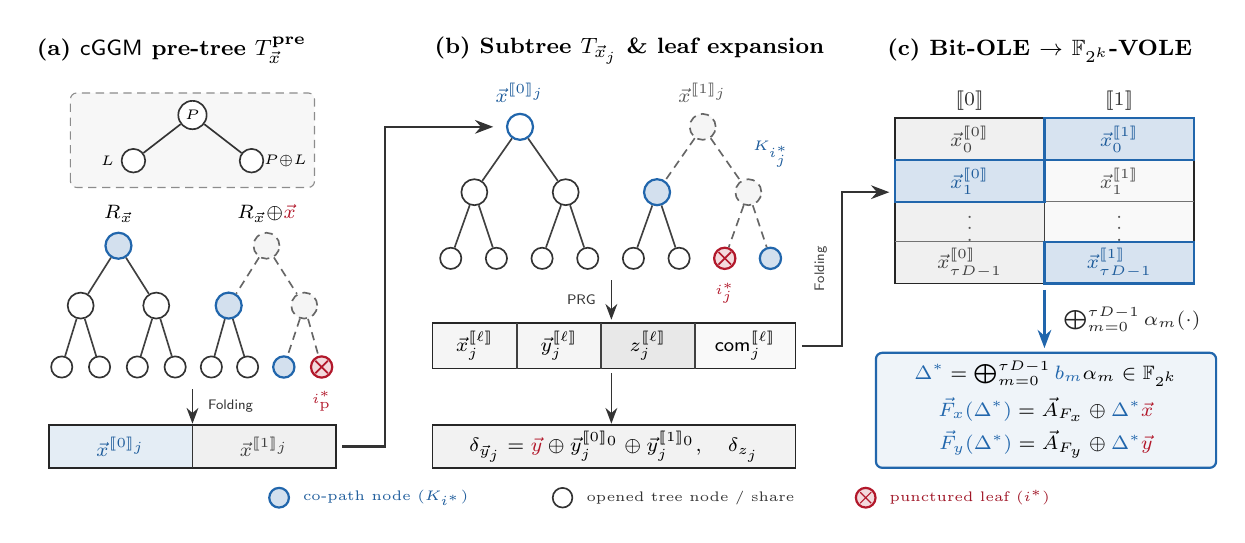
\begin{tikzpicture}[
    >=Stealth,
    font=\footnotesize,
    tnode/.style={circle, draw=black!80, semithick, fill=white, minimum size=3.3mm, inner sep=0pt},
    copath/.style={circle, draw=accentblue, thick, fill=accentblue!20, minimum size=3.3mm, inner sep=0pt},
    missnode/.style={circle, draw=black!60, semithick, densely dashed, fill=gray!8, minimum size=3.3mm, inner sep=0pt},
    punctleaf/.style={circle, draw=accentred, thick, fill=accentred!16, minimum size=3.3mm, inner sep=0pt},
    matborder/.style={semithick, draw=black!85}
]
    % =========================================================================
    % STAGE (a): cGGM Split & Pre-Tree T_x^{pre} (x = 0.00 .. 4.15)
    % =========================================================================
    \node[anchor=west, font=\footnotesize\bfseries] at (0.00, 4.52) {(a) $\cGGM$ pre-tree $T_{\vec{x}}^{\text{pre}}$};

    % Clean cGGM split gadget (top center of column a)
    \fill[gray!6, rounded corners=0.8mm] (0.55, 2.78) rectangle (3.65, 3.98);
    \draw[black!45, densely dashed, rounded corners=0.8mm] (0.55, 2.78) rectangle (3.65, 3.98);
    \node[tnode, minimum size=3.6mm, font=\tiny] (P0) at (2.10, 3.70) {$P$};
    \node[tnode, minimum size=3.0mm] (L0) at (1.35, 3.12) {};
    \node[tnode, minimum size=3.0mm] (R0) at (2.85, 3.12) {};
    \draw[semithick, black!80] (P0) -- (L0) (P0) -- (R0);
    \node[font=\tiny] at (1.02, 3.12) {$L$};
    \node[font=\tiny] at (3.28, 3.12) {$P{\oplus}L$};

    % Pre-tree level 1..tau
    \node[copath] (PT10) at (1.16, 2.04) {};
    \node[missnode] (PT11) at (3.04, 2.04) {};
    \node[above=1pt, font=\scriptsize] at (1.16, 2.18) {$R_{\vec{x}}$};
    \node[above=1pt, font=\scriptsize] at (3.04, 2.18) {$R_{\vec{x}}{\oplus}{\color{accentred}\vec{x}}$};

    % Pre-tree level 2
    \node[tnode] (PT20) at (0.68, 1.28) {};
    \node[tnode] (PT21) at (1.64, 1.28) {};
    \node[copath] (PT22) at (2.56, 1.28) {};
    \node[missnode] (PT23) at (3.52, 1.28) {};
    \draw[semithick, black!75] (PT10) -- (PT20) (PT10) -- (PT21);
    \draw[semithick, black!60, densely dashed] (PT11) -- (PT22) (PT11) -- (PT23);

    % Pre-tree leaves (8 leaves representing 2^\tau)
    \foreach \idx/\xpos/\sty in {0/0.44/tnode, 1/0.92/tnode, 2/1.40/tnode, 3/1.88/tnode, 4/2.34/tnode, 5/2.80/tnode, 6/3.26/copath, 7/3.74/punctleaf} {
        \node[\sty, minimum size=2.7mm] (PTL\idx) at (\xpos, 0.50) {};
    }
    \draw[semithick, black!75] (PT20) -- (PTL0) (PT20) -- (PTL1) (PT21) -- (PTL2) (PT21) -- (PTL3) (PT22) -- (PTL4) (PT22) -- (PTL5);
    \draw[semithick, black!60, densely dashed] (PT23) -- (PTL6) (PT23) -- (PTL7);
    \draw[accentred, semithick] ($(PTL7.center)+(-0.8mm,-0.8mm)$) -- ($(PTL7.center)+(0.8mm,0.8mm)$)
                                ($(PTL7.center)+(-0.8mm,0.8mm)$) -- ($(PTL7.center)+(0.8mm,-0.8mm)$);
    \node[below=1pt, font=\tiny, text=accentred] at (PTL7.south) {$i^*_{\text{p}}$};

    % Folded pre-tree bar
    \draw[->, semithick, black!80] (2.10, 0.22) -- node[right=2pt, font=\tiny] {$\Folding$} (2.10, -0.22);
    \fill[accentblue!12] (0.28, -0.78) rectangle (2.10, -0.24);
    \fill[gray!12] (2.10, -0.78) rectangle (3.92, -0.24);
    \draw[matborder] (0.28, -0.78) rectangle (3.92, -0.24);
    \draw[semithick, black!80] (2.10, -0.78) -- (2.10, -0.24);
    \node[font=\scriptsize, text=accentblue!90!black] at (1.19, -0.51) {$\vec{x}^{\share{0}_j}$};
    \node[font=\scriptsize, text=black!75] at (3.01, -0.51) {$\vec{x}^{\share{1}_j}$};

    % Connector (a) -> (b)
    \draw[->, thick, black!80] (4.00, -0.51) -- (4.55, -0.51) -- (4.55, 3.55) -- (5.92, 3.55);

    % =========================================================================
    % STAGE (b): Second-Layer Tree T_{x_j} & Leaf Expansion (x = 5.05 .. 9.85)
    % =========================================================================
    \node[anchor=west, font=\footnotesize\bfseries] at (5.05, 4.52) {(b) Subtree $T_{\vec{x}_j}$ \& leaf expansion};

    % Subtree level 1
    \node[tnode, draw=accentblue, thick] (ST10) at (6.26, 3.55) {};
    \node[missnode] (ST11) at (8.58, 3.55) {};
    \node[above=1pt, font=\scriptsize, text=accentblue!90!black] at (6.26, 3.70) {$\vec{x}^{\share{0}_j}$};
    \node[above=1pt, font=\scriptsize, text=black!65] at (8.58, 3.70) {$\vec{x}^{\share{1}_j}$};

    % Subtree level 2
    \node[tnode] (ST20) at (5.68, 2.72) {};
    \node[tnode] (ST21) at (6.84, 2.72) {};
    \node[copath] (ST22) at (8.00, 2.72) {};
    \node[missnode] (ST23) at (9.16, 2.72) {};
    \draw[semithick, black!75] (ST10) -- (ST20) (ST10) -- (ST21);
    \draw[semithick, black!60, densely dashed] (ST11) -- (ST22) (ST11) -- (ST23);

    % Subtree level D leaves (8 leaves representing 2^D)
    \foreach \idx/\xpos/\sty in {0/5.38/tnode, 1/5.96/tnode, 2/6.54/tnode, 3/7.12/tnode, 4/7.70/tnode, 5/8.28/tnode, 6/8.86/punctleaf, 7/9.44/copath} {
        \node[\sty, minimum size=2.7mm] (STL\idx) at (\xpos, 1.88) {};
    }
    \draw[semithick, black!75] (ST20) -- (STL0) (ST20) -- (STL1) (ST21) -- (STL2) (ST21) -- (STL3) (ST22) -- (STL4) (ST22) -- (STL5);
    \draw[semithick, black!60, densely dashed] (ST23) -- (STL6) (ST23) -- (STL7);
    \draw[accentred, semithick] ($(STL6.center)+(-0.8mm,-0.8mm)$) -- ($(STL6.center)+(0.8mm,0.8mm)$)
                                ($(STL6.center)+(-0.8mm,0.8mm)$) -- ($(STL6.center)+(0.8mm,-0.8mm)$);
    \node[below=1pt, font=\tiny, text=accentred] at (STL6.south) {$i^*_j$};
    \node[font=\tiny, text=accentblue!90!black] at (9.45, 3.20) {$K_{i^*_j}$};

    % Expansion arrow to 4-field leaf strip
    \draw[->, semithick, black!80] (7.42, 1.60) -- node[left=2pt, font=\tiny] {$\PRG$} (7.42, 1.10);

    % 4-field expanded leaf strip
    \fill[gray!8]  (5.15, 0.48) rectangle (6.22, 1.06);
    \fill[gray!8]  (6.22, 0.48) rectangle (7.29, 1.06);
    \fill[gray!18] (7.29, 0.48) rectangle (8.48, 1.06);
    \fill[gray!5]  (8.48, 0.48) rectangle (9.76, 1.06);
    \draw[matborder] (5.15, 0.48) rectangle (9.76, 1.06);
    \draw[semithick, black!75] (6.22, 0.48) -- (6.22, 1.06) (7.29, 0.48) -- (7.29, 1.06) (8.48, 0.48) -- (8.48, 1.06);
    \node[font=\scriptsize] at (5.685, 0.77) {$\vec{x}_j^{\share{\ell}}$};
    \node[font=\scriptsize] at (6.755, 0.77) {$\vec{y}_j^{\share{\ell}}$};
    \node[font=\scriptsize] at (7.885, 0.77) {$z_j^{\share{\ell}}$};
    \node[font=\scriptsize] at (9.120, 0.77) {$\com_j^{\share{\ell}}$};

    % Per-tree offsets box
    \draw[->, semithick, black!80] (7.42, 0.42) -- (7.42, -0.22);
    \fill[gray!10] (5.15, -0.78) rectangle (9.76, -0.24);
    \draw[matborder] (5.15, -0.78) rectangle (9.76, -0.24);
    \node[font=\scriptsize] at (7.455, -0.51) {$\delta_{\vec{y}_j} = {\color{accentred}\vec{y}} \oplus \vec{y}_j^{\share{0}_0} \oplus \vec{y}_j^{\share{1}_0},\quad \delta_{z_j}$};

    % Connector (b) -> (c)
    \draw[->, thick, black!80] (9.84, 0.77) -- (10.35, 0.77) -- (10.35, 2.72) -- (10.95, 2.72);
    \node[above, font=\tiny, text=black!75, rotate=90] at (10.28, 1.75) {$\Folding$};

    % =========================================================================
    % STAGE (c): Hypercube Bit-OLE -> F_{2^k} VOLE (x = 10.80 .. 15.10)
    % =========================================================================
    \node[anchor=west, font=\footnotesize\bfseries] at (10.80, 4.52) {(c) Bit-OLE $\to$ $\Ftwok$-VOLE};

    % Hypercube 2-column share matrix
    \node[font=\scriptsize, text=black!80] at (11.97, 3.88) {$\share{0}$};
    \node[font=\scriptsize, text=black!80] at (13.87, 3.88) {$\share{1}$};

    % Base background of 2 columns (x: 11.02..12.92 and 12.92..14.82, y: 1.56..3.66)
    \fill[gray!12] (11.02, 1.56) rectangle (12.92, 3.66);
    \fill[gray!5]  (12.92, 1.56) rectangle (14.82, 3.66);

    % Highlighted opened branch cells b_m = 1 \oplus bit_i(i^*_j)
    \fill[accentblue!18] (12.92, 3.13) rectangle (14.82, 3.66);
    \fill[accentblue!18] (11.02, 2.60) rectangle (12.92, 3.13);
    \fill[accentblue!18] (12.92, 1.56) rectangle (14.82, 2.09);

    \draw[matborder] (11.02, 1.56) rectangle (14.82, 3.66);
    \draw[semithick, black!75] (12.92, 1.56) -- (12.92, 3.66);
    \draw[thin, black!55] (11.02, 3.13) -- (14.82, 3.13)
                          (11.02, 2.60) -- (14.82, 2.60)
                          (11.02, 2.09) -- (14.82, 2.09);
    \draw[thick, accentblue] (12.92, 3.13) rectangle (14.82, 3.66);
    \draw[thick, accentblue] (11.02, 2.60) rectangle (12.92, 3.13);
    \draw[thick, accentblue] (12.92, 1.56) rectangle (14.82, 2.09);

    \node[font=\scriptsize, text=black!75] at (11.97, 3.39) {$\vec{x}_0^{\share{0}}$};
    \node[font=\scriptsize, text=accentblue!90!black] at (13.87, 3.39) {$\vec{x}_0^{\share{1}}$};
    \node[font=\scriptsize, text=accentblue!90!black] at (11.97, 2.86) {$\vec{x}_1^{\share{0}}$};
    \node[font=\scriptsize, text=black!70] at (13.87, 2.86) {$\vec{x}_1^{\share{1}}$};
    \node[font=\scriptsize, text=black!65] at (11.97, 2.36) {$\vdots$};
    \node[font=\scriptsize, text=black!65] at (13.87, 2.36) {$\vdots$};
    \node[font=\scriptsize, text=black!75] at (11.97, 1.82) {$\vec{x}_{\tau D-1}^{\share{0}}$};
    \node[font=\scriptsize, text=accentblue!90!black] at (13.87, 1.82) {$\vec{x}_{\tau D-1}^{\share{1}}$};

    % Lifting arrow with \alpha_m
    \draw[->, thick, accentblue] (12.92, 1.48) -- node[right=3pt, font=\scriptsize, text=black!85] {$\bigoplus_{m=0}^{\tau D-1} \alpha_m (\cdot)$} (12.92, 0.74);

    % Resulting F_{2^k}-VOLE box
    \fill[accentblue!7, rounded corners=0.8mm] (10.78, -0.78) rectangle (15.10, 0.68);
    \draw[thick, accentblue, rounded corners=0.8mm] (10.78, -0.78) rectangle (15.10, 0.68);
    \node[font=\scriptsize] at (12.94, 0.42) {${\color{accentblue}\Delta^*} = \bigoplus_{m=0}^{\tau D-1} {\color{accentblue}b_m}\alpha_m \in \Ftwok$};
    \node[font=\scriptsize] at (12.94, -0.04) {${\color{accentblue}\vec{F}_x(\Delta^*)} = \vec{A}_{F_x} \oplus {\color{accentblue}\Delta^*}{\color{accentred}\vec{x}}$};
    \node[font=\scriptsize] at (12.94, -0.48) {${\color{accentblue}\vec{F}_y(\Delta^*)} = \vec{A}_{F_y} \oplus {\color{accentblue}\Delta^*}{\color{accentred}\vec{y}}$};

    % Clean bottom legend bar
    \node[copath, minimum size=2.5mm] at (3.20, -1.16) {};
    \node[anchor=west, font=\tiny, text=accentblue!90!black] at (3.38, -1.16) {co-path node ($K_{i^*}$)};
    \node[tnode, minimum size=2.5mm] at (6.80, -1.16) {};
    \node[anchor=west, font=\tiny, text=black!80] at (6.98, -1.16) {opened tree node / share};
    \node[punctleaf, minimum size=2.5mm] (legp) at (10.65, -1.16) {};
    \draw[accentred, thin] ($(legp.center)+(-0.7mm,-0.7mm)$) -- ($(legp.center)+(0.7mm,0.7mm)$)
                           ($(legp.center)+(-0.7mm,0.7mm)$) -- ($(legp.center)+(0.7mm,-0.7mm)$);
    \node[anchor=west, font=\tiny, text=accentred!90!black] at (10.83, -1.16) {punctured leaf ($i^*$)};
\end{tikzpicture}
\caption{VOLE-in-the-Head architecture of $\SBCVOLE$~\cite{HJ25}. \textbf{(a)}~An XOR-preserving $\cGGM$ pre-tree $T_{\vec{x}}^{\text{pre}}$ splits $(R_{\vec{x}}, R_{\vec{x}} \oplus \vec{x})$ into $2^\tau$ leaves and folds them into $\tau$ binary root sharings $(\vec{x}^{\share{0}_j}, \vec{x}^{\share{1}_j})$ of $\vec{x}$. \textbf{(b)}~Each second-layer tree $T_{\vec{x}_j}$ ($N = 2^D$ leaves) expands every leaf into $(\vec{x}_j^{\share{\ell}}, \vec{y}_j^{\share{\ell}}, z_j^{\share{\ell}}, \com_j^{\share{\ell}})$, using public offsets $(\delta_{\vec{y}_j}, \delta_{z_j})$ to align $(\vec{y}, z)$ across trees; revealing the sibling co-path $K_{i^*_j}$ (blue) opens $2^D - 1$ leaves while hiding leaf $i^*_j$ (red). \textbf{(c)}~Hypercube folding turns the opened half-cubes $b_m = 1 \oplus \mathsf{bit}_i(i^*_j)$ into $\tau D$ bit-level OLEs $f_m(b_m) = \vec{x}_m^{\share{0}} \oplus b_m\vec{x}$, whose $\alpha_m$-weighted sum yields the $\Ftwok$-VOLE evaluations $\vec{F}_x(\Delta^*)$ and $\vec{F}_y(\Delta^*)$.}
\label{fig:vole-architecture}
\end{figure}

\subsection{Verification Polynomial and Cross-Tree Consistency}
Using the first-challenge weights $(\alpha_m)_{m \in [\tau D]} \in (\Ftwok)^{\tau D}$, the signer forms the constant VOLE mask vectors $\vec{A}_{F_x}, \vec{A}_{F_y} \in (\Ftwok)^{n-2}$ from the $0$-side hypercube shares~\cite{HJ25}:
\begin{equation}
\label{eq:AFx-AFy}
\vec{A}_{F_x} \leftarrow \bigoplus_{j=0}^{\tau-1} \bigoplus_{i=jD}^{(j+1)D-1} \alpha_i \, \vec{x}_j^{\share{0}_{i - jD}}, \qquad
\vec{A}_{F_y} \leftarrow \bigoplus_{j=0}^{\tau-1} \bigoplus_{i=jD}^{(j+1)D-1} \alpha_i \, \vec{y}_j^{\share{0}_{i - jD}}.
\end{equation}
For any formal evaluation point $\Delta \in \Ftwok$, the underlying VOLE vector polynomials are the degree-$1$ affine functions
\begin{equation}
\label{eq:Fx-Fy-poly}
\vec{F}_x(\Delta) = \vec{A}_{F_x} \oplus \Delta \cdot \vec{x} \in (\Ftwok)^{n-2}, \qquad
\vec{F}_y(\Delta) = \vec{A}_{F_y} \oplus \Delta \cdot \vec{y} \in (\Ftwok)^{n-2}.
\end{equation}

To verify that $(\vec{x}', \vec{y}') = ((\vec{x}, 1, 0), (\vec{y}, 0, 1))$ satisfies the normalised bilinear collision relation~\eqref{eq:sbc}, the protocol embeds $\vec{F}_x(\Delta)$ and $\vec{F}_y(\Delta)$ into length-$n$ vectors and evaluates the bilinear determinant polynomial $\Phi(\Delta) = A \oplus B\Delta \oplus C\Delta^2 \in \Ftwok[\Delta]$, whose quadratic coefficient is
\begin{equation}
\label{eq:C-coeff}
C = \left(\vec{u} \cdot \begin{pmatrix} \vec{x} \\ 1 \\ 0 \end{pmatrix}\right) \left(\vec{v} \cdot \begin{pmatrix} \vec{y} \\ 0 \\ 1 \end{pmatrix}\right) \oplus \left(\vec{u} \cdot \begin{pmatrix} \vec{y} \\ 0 \\ 1 \end{pmatrix}\right) \left(\vec{v} \cdot \begin{pmatrix} \vec{x} \\ 1 \\ 0 \end{pmatrix}\right).
\end{equation}
By Definition~\ref{def:sbc}, $C = 0$ if and only if $(\vec{x}', \vec{y}') \in \NSBC[\vec{u}, \vec{v}]$, in which case $\Phi(\Delta)$ reduces to the degree-$1$ affine polynomial $\Phi(\Delta) = A \oplus B\Delta$. Writing $\eta \in \{0, 1\}$ for the normalisation-coordinate mask padding indicator, the constant term $A \in \Ftwok$ and linear slope $B \in \Ftwok$ are given by~\cite{HJ25}:
\begin{align}
A &\leftarrow \left(\vec{u} \cdot \begin{pmatrix} \vec{A}_{F_x} \\ \eta \\ 0 \end{pmatrix}\right) \left(\vec{v} \cdot \begin{pmatrix} \vec{A}_{F_y} \\ 0 \\ \eta \end{pmatrix}\right) \oplus \left(\vec{u} \cdot \begin{pmatrix} \vec{A}_{F_y} \\ 0 \\ \eta \end{pmatrix}\right) \left(\vec{v} \cdot \begin{pmatrix} \vec{A}_{F_x} \\ \eta \\ 0 \end{pmatrix}\right), \label{eq:A-def} \\[4pt]
B &\leftarrow \left(\vec{v} \cdot \begin{pmatrix} \vec{A}_{F_y} \\ 0 \\ \eta \end{pmatrix}\right) \left(\vec{u} \cdot \begin{pmatrix} \vec{x} \\ 1 \\ 0 \end{pmatrix}\right) \oplus \left(\vec{u} \cdot \begin{pmatrix} \vec{A}_{F_x} \\ \eta \\ 0 \end{pmatrix}\right) \left(\vec{v} \cdot \begin{pmatrix} \vec{y} \\ 0 \\ 1 \end{pmatrix}\right) \nonumber \\
&\quad \oplus \left(\vec{u} \cdot \begin{pmatrix} \vec{A}_{F_y} \\ 0 \\ \eta \end{pmatrix}\right) \left(\vec{v} \cdot \begin{pmatrix} \vec{x} \\ 1 \\ 0 \end{pmatrix}\right) \oplus \left(\vec{v} \cdot \begin{pmatrix} \vec{A}_{F_x} \\ \eta \\ 0 \end{pmatrix}\right) \left(\vec{u} \cdot \begin{pmatrix} \vec{y} \\ 0 \\ 1 \end{pmatrix}\right). \label{eq:B-def}
\end{align}

\paragraph{Normalisation-Coordinate Padding ($\eta \in \{0, 1\}$).}
Setting $\eta = 1$ in~\eqref{eq:A-def}--\eqref{eq:B-def} places $(1, 0)$ and $(0, 1)$ in the last two coordinates of $\vec{A}_{F_x}, \vec{A}_{F_y}$ as printed in~\cite[Figure~5]{HJ25}, whereas setting $\eta = 0$ shares the fixed coordinates homogeneously as $0 \oplus 1 \cdot \Delta$ (so $(\vec{F}_x(\Delta), \Delta, 0)$ and $(\vec{F}_y(\Delta), 0, \Delta)$ scale uniformly with $\Delta$), as implemented in the authors' official reference artifact. Carrying $\eta \in \{0, 1\}$ throughout Section~\ref{sec:key-recovery} covers both conventions simultaneously; $\eta$ shifts only a known public constant in the linear coefficients and has no effect on the quadratic cancellation.

In addition to $A$ and $B$, the signer computes the cross-tree consistency responses~\cite{HJ25}:
\begin{equation}
\label{eq:b-aj}
b \leftarrow z \oplus \vec{y} \cdot \vec{\mu} \in \Ftwok, \qquad
a^{(j)} \leftarrow \vec{A}_{F_y}^{(j)} \cdot \vec{\mu} \oplus A_{F_z}^{(j)} \in \Ftwok \quad (j \in [\tau]),
\end{equation}
where $\vec{A}_{F_y}^{(j)} = \bigoplus_{i=jD}^{(j+1)D-1} \alpha_i \vec{y}_j^{\share{0}_{i-jD}}$ and $A_{F_z}^{(j)} = \bigoplus_{i=jD}^{(j+1)D-1} \alpha_i z_j^{\share{0}_{i-jD}}$, corresponding to the per-tree VOLE polynomials $\vec{F}_y^{(j)}(\Delta_j) = \vec{A}_{F_y}^{(j)} \oplus \Delta_j \vec{y}$ and $Z^{(j)}(\Delta_j) = A_{F_z}^{(j)} \oplus \Delta_j z$ at $\Delta_j = \bigoplus_{i=jD}^{(j+1)D-1} b_i \alpha_i$.

\subsection{Five-Pass Identification Protocol and Fiat--Shamir Signature}
\label{subsec:fs-vulnerability}
Figure~\ref{fig:protocol-fiat-shamir} illustrates the five-pass interactive identification protocol between Prover $\mathcal{P}(\pk, \sk)$ and Verifier $\mathcal{V}(\pk)$, together with its compilation into a non-interactive signature $\sigma$~\cite[Sections~4--5]{HJ25}.

\paragraph{Interactive Five-Pass Identification Protocol (Figure~\ref{fig:protocol-fiat-shamir}a, Left).}
The interactive proof of knowledge of $(\vec{x}', \vec{y}') \in \NSBC[\vec{u}, \vec{v}]$ proceeds across five passes:
\begin{itemize}[leftmargin=2em, itemsep=2.5pt]
    \item \textbf{Pass~1 (Commitment, $\mathcal{P} \to \mathcal{V}$):} $\mathcal{P}$ samples $R_{\vec{x}} \xleftarrow{\$} \Ftwo^{n-2}$ and $\salt \xleftarrow{\$} \{0,1\}^{2\lambda}$, generates the correlated $\cGGM$ forest $(T_{\vec{x}}^{\text{pre}}, T_{\vec{x}_0}, \dots, T_{\vec{x}_{\tau-1}})$, expands and folds all leaf shares, computes the alignment offsets $(\delta_{\vec{y}_j})_{j \in [\tau]}$ and $(\delta_{z_j})_{j \in [\tau]^*}$ via~\eqref{eq:offsets} as well as the global commitment digest $h_{\com}$, and sends $\big(h_{\com}, \salt, (\delta_{\vec{y}_j})_{j \in [\tau]}, (\delta_{z_j})_{j \in [\tau]^*}, (X_j)_{j \in [\tau]}\big)$ to $\mathcal{V}$ (with $(X_j)_{j \in [\tau]}$ omitted in $\SBCVOLEM$).
    \item \textbf{Pass~2 (First Challenge, $\mathcal{V} \to \mathcal{P}$):} $\mathcal{V}$ samples the cross-tree consistency vector $\vec{\mu} \xleftarrow{\$} (\Ftwok)^{n-2}$ and the VOLE lifting weights $(\alpha_m)_{m \in [\tau D]} \xleftarrow{\$} (\Ftwok)^{\tau D}$, and sends $\big(\vec{\mu}, (\alpha_m)_{m \in [\tau D]}\big)$ to $\mathcal{P}$.
    \item \textbf{Pass~3 (First Response, $\mathcal{P} \to \mathcal{V}$):} From the $0$-side hypercube shares and the Pass~2 challenges, $\mathcal{P}$ computes the VOLE mask vectors $(\vec{A}_{F_x}, \vec{A}_{F_y})$ via~\eqref{eq:AFx-AFy}, evaluates the verification coefficients $(A, B) \in \Ftwok \times \Ftwok$ via~\eqref{eq:A-def}--\eqref{eq:B-def} and the consistency responses $b \in \Ftwok$ and $(a^{(j)})_{j \in [\tau]} \in (\Ftwok)^\tau$ via~\eqref{eq:b-aj}, and sends $\big(A, B, (a^{(j)})_{j \in [\tau]}, b\big)$ to $\mathcal{V}$.
    \item \textbf{Pass~4 (Second Challenge, $\mathcal{V} \to \mathcal{P}$):} $\mathcal{V}$ samples one punctured leaf index $i^*_j \xleftarrow{\$} [2^D]$ for each tree $j \in [\tau]$, implicitly fixing the complementary branch bits $b_m = 1 \oplus \mathsf{bit}_i(i^*_j)$ and the evaluation points $(\Delta^*_j)_{j \in [\tau]}$ and $\Delta^* = \bigoplus_{j=0}^{\tau-1} \Delta^*_j$, and sends $(i^*_j)_{j \in [\tau]}$ to $\mathcal{P}$.
    \item \textbf{Pass~5 (Second Response and Verification, $\mathcal{P} \to \mathcal{V}$):} $\mathcal{P}$ forms the pre-tree index $i^*_{\text{p}} = \sum_{j=0}^{\tau-1} \mathsf{bit}_{D-1}(i^*_j) 2^j$ and sends the punctured forest keys $(K_{i^*_{\text{p}}}, K_{i^*_0, \dots, i^*_{\tau-1}})$ to $\mathcal{V}$ (aborting and restarting in $\SBCVOLEM$ if any $i^*_j$ hits a commitment extremum). Using the opened leaves and Pass~1 offsets, $\mathcal{V}$ recomputes $h'_{\com}$, $(\vec{F}_y^{(j)}(\Delta^*_j), Z^{(j)}(\Delta^*_j))_{j \in [\tau]}$, and $(\vec{F}_x(\Delta^*), \vec{F}_y(\Delta^*))$, and accepts if and only if $h'_{\com} = h_{\com}$, $Z^{(j)}(\Delta^*_j) \oplus \vec{F}_y^{(j)}(\Delta^*_j) \cdot \vec{\mu} = a^{(j)} \oplus b\Delta^*_j$ for all $j \in [\tau]$, and $\Phi(\Delta^*) = A \oplus B\Delta^*$.
\end{itemize}

\paragraph{Non-Interactive Fiat--Shamir Signature (Figure~\ref{fig:protocol-fiat-shamir}a, Right \& \ref{fig:protocol-fiat-shamir}b).}
Applying the five-pass Fiat--Shamir transform~\cite{FS86} to sign a message $\msg \in \{0,1\}^*$ replaces $\mathcal{V}$'s two interactive challenges with random-oracle digests expanded via PRGs:
\begin{itemize}[leftmargin=2em, itemsep=2.5pt]
    \item \textbf{First Challenge Digest ($H_0 \to \PRG_0$):} After running Pass~1, the signer hashes $\msg$ and the commitment transcript into
    \begin{equation}
    \label{eq:h0}
    h_0 \leftarrow H_0\big(\msg, h_{\com}, \salt, (\delta_{\vec{y}_j}, \delta_{z_j})_{j \in [\tau]}, (X_j)_{j \in [\tau]}\big),
    \end{equation}
    and expands $\big(\vec{\mu}, (\alpha_m)_{m \in [\tau D]}\big) \leftarrow \PRG_0(h_0)$ locally in place of Pass~2.
    \item \textbf{Second Challenge Digest ($H_1 \to \PRG_1$):} After computing the Pass~3 responses $\big(A, B, (a^{(j)})_{j \in [\tau]}, b\big)$, the signer hashes them together with $h_0$ into
    \begin{equation}
    \label{eq:h1}
    h_1 \leftarrow H_1\Big(\msg, h_{\com}, \salt, (\delta_{\vec{y}_j}, \delta_{z_j})_{j \in [\tau]}, h_0, A, B, (a^{(j)})_{j \in [\tau]}, b\Big),
    \end{equation}
    and derives the punctured leaf indices $(i^*_j)_{j \in [\tau]} \leftarrow \PRG_1(h_1)$ in place of Pass~4.
    \item \textbf{Transcript Compression and Signature Format:} During verification, $\mathcal{V}$ derives $(i^*_j)_{j \in [\tau]} \leftarrow \PRG_1(h_1)$, opens the punctured forest to recover $h'_{\com}$, $h'_0$, and the VOLE evaluations, reconstructs $A' \leftarrow \Phi(\Delta^*) \oplus B\Delta^*$ and $a'^{(j)} \leftarrow Z^{(j)}(\Delta^*_j) \oplus \vec{F}_y^{(j)}(\Delta^*_j) \cdot \vec{\mu} \oplus b\Delta^*_j$ ($j \in [\tau]$), and checks $h'_1 = h_1$. Because $h_0$, $A$, and $(a^{(j)})_{j \in [\tau]}$ are deterministically recomputed by $\mathcal{V}$, they are omitted from transmission, yielding the signature tuple
    \begin{equation}
    \label{eq:sigma}
    \sigma = \Big(h_1, \, \salt, \, (\delta_{\vec{y}_j})_{j \in [\tau]}, \, (\delta_{z_j})_{j \in [\tau]^*}, \, B, \, b, \, K_{i^*_{\text{p}}}, \, K_{i^*_0, \dots, i^*_{\tau-1}}, \, (X_j)_{j \in [\tau]}\Big),
    \end{equation}
    where $(X_j)_{j \in [\tau]}$ is omitted in the MinMax variant $\SBCVOLEM$.
\end{itemize}

\begin{figure}[t]
\centering
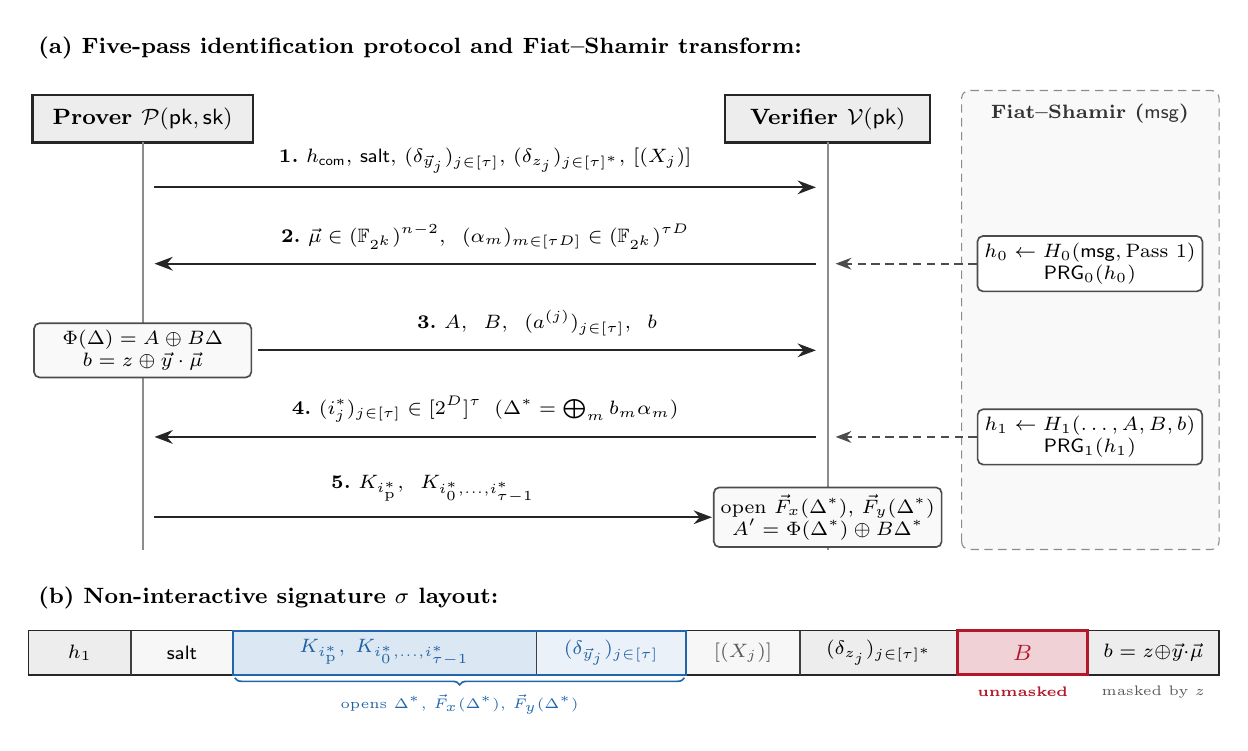
\begin{tikzpicture}[
    >=Stealth,
    font=\footnotesize,
    rolebox/.style={rectangle, draw=black!85, thick, fill=gray!14, minimum height=6.0mm, inner sep=2pt, font=\footnotesize\bfseries},
    statebox/.style={rectangle, draw=black!70, semithick, fill=gray!5, rounded corners=0.7mm, inner sep=2.5pt, align=center, font=\scriptsize},
    fsbox/.style={rectangle, draw=black!70, semithick, fill=white, rounded corners=0.7mm, inner sep=2.5pt, align=center, font=\scriptsize},
    msgarrow/.style={->, >=Stealth, thick, draw=black!85},
    matborder/.style={semithick, draw=black!85}
]
    % =========================================================================
    % PART (a): 5-Pass Interactive Protocol + Fiat--Shamir Sidecar
    % =========================================================================
    \node[anchor=west, font=\footnotesize\bfseries] at (0.00, 6.92) {(a) Five-pass identification protocol and Fiat--Shamir transform:};

    % Fiat-Shamir background container on the right (x: 11.85 .. 15.12)
    \fill[gray!5, rounded corners=1.0mm] (11.85, 0.55) rectangle (15.12, 6.38);
    \draw[black!45, densely dashed, rounded corners=1.0mm] (11.85, 0.55) rectangle (15.12, 6.38);
    \node[font=\scriptsize\bfseries, text=black!80] at (13.48, 6.08) {Fiat--Shamir ($\msg$)};

    % Prover (x = 1.45) and Verifier (x = 10.15)
    \node[rolebox, minimum width=2.80cm] (Phdr) at (1.45, 6.02) {Prover $\mathcal{P}(\pk, \sk)$};
    \node[rolebox, minimum width=2.60cm] (Vhdr) at (10.15, 6.02) {Verifier $\mathcal{V}(\pk)$};

    % Clean lifelines
    \draw[black!45, semithick] (1.45, 5.72) -- (1.45, 0.55);
    \draw[black!45, semithick] (10.15, 5.72) -- (10.15, 0.55);

    % --- PASS 1: Commitment (y = 5.15) ---
    \draw[msgarrow] (1.60, 5.15) -- node[above=1.5pt, font=\scriptsize] {\textbf{1.}\ $h_{\com},\, \salt,\, (\delta_{\vec{y}_j})_{j\in[\tau]},\, (\delta_{z_j})_{j\in[\tau]^*},\, [(X_j)]$} (10.00, 5.15);

    % --- PASS 2: Challenge 1 (y = 4.18) ---
    \draw[msgarrow] (10.00, 4.18) -- node[above=1.5pt, font=\scriptsize] {\textbf{2.}\ $\vec{\mu} \in (\Ftwok)^{n-2},\;\; (\alpha_m)_{m\in[\tau D]} \in (\Ftwok)^{\tau D}$} (1.60, 4.18);
    \node[fsbox, minimum width=2.82cm] (FSh0) at (13.48, 4.18) {$h_0 \leftarrow H_0(\msg, \text{Pass 1})$\\$\PRG_0(h_0)$};
    \draw[->, densely dashed, semithick, black!70] (FSh0.west) -- (10.25, 4.18);

    % --- PASS 3: Response 1 (y = 3.08) ---
    \node[statebox, minimum width=2.76cm] (P3) at (1.45, 3.08) {$\Phi(\Delta) = A \oplus B\Delta$\\$b = z \oplus \vec{y} \cdot \vec{\mu}$};
    \draw[msgarrow] (2.92, 3.08) -- node[above=1.5pt, font=\scriptsize] {\textbf{3.}\ $A,\;\; B,\;\; (a^{(j)})_{j\in[\tau]},\;\; b$} (10.00, 3.08);

    % --- PASS 4: Challenge 2 (y = 1.98) ---
    \draw[msgarrow] (10.00, 1.98) -- node[above=1.5pt, font=\scriptsize] {\textbf{4.}\ $(i^*_j)_{j\in[\tau]} \in [2^D]^\tau \;\;(\Delta^* = \bigoplus_m b_m\alpha_m)$} (1.60, 1.98);
    \node[fsbox, minimum width=2.82cm] (FSh1) at (13.48, 1.98) {$h_1 \leftarrow H_1(\dots, A, B, b)$\\$\PRG_1(h_1)$};
    \draw[->, densely dashed, semithick, black!70] (FSh1.west) -- (10.25, 1.98);

    % --- PASS 5: Response 2 / Punctured Opening (y = 0.96) ---
    \draw[msgarrow] (1.60, 0.96) -- node[above=1.5pt, font=\scriptsize] {\textbf{5.}\ $K_{i^*_{\text{p}}},\;\; K_{i^*_0, \dots, i^*_{\tau-1}}$} (8.68, 0.96);
    \node[statebox, minimum width=2.70cm] at (10.15, 0.96) {open $\vec{F}_x(\Delta^*),\, \vec{F}_y(\Delta^*)$\\$A' = \Phi(\Delta^*) \oplus B\Delta^*$};

    % =========================================================================
    % PART (b): Non-Interactive Signature \sigma Wire Layout
    % =========================================================================
    \node[anchor=west, font=\footnotesize\bfseries] at (0.00, -0.06) {(b) Non-interactive signature $\sigma$ layout:};

    \begin{scope}[yshift=-1.04cm]
        \fill[gray!14]       (0.00, 0.00) rectangle (1.30, 0.56);
        \fill[gray!6]        (1.30, 0.00) rectangle (2.60, 0.56);
        \fill[accentblue!16] (2.60, 0.00) rectangle (6.45, 0.56);
        \fill[accentblue!9]  (6.45, 0.00) rectangle (8.35, 0.56);
        \fill[gray!6]        (8.35, 0.00) rectangle (9.80, 0.56);
        \fill[gray!14]       (9.80, 0.00) rectangle (11.80, 0.56);
        \fill[accentred!20]  (11.80, 0.00) rectangle (13.45, 0.56);
        \fill[gray!14]       (13.45, 0.00) rectangle (15.12, 0.56);

        \draw[matborder] (0.00, 0.00) rectangle (15.12, 0.56);
        \foreach \x in {1.30, 2.60, 6.45, 8.35, 9.80, 11.80, 13.45} {
            \draw[semithick, black!75] (\x, 0.00) -- (\x, 0.56);
        }
        \draw[thick, accentblue] (2.60, 0.00) rectangle (8.35, 0.56);
        \draw[very thick, accentred] (11.80, 0.00) rectangle (13.45, 0.56);

        \node[font=\scriptsize] at (0.650, 0.28) {$h_1$};
        \node[font=\scriptsize] at (1.950, 0.28) {$\salt$};
        \node[font=\scriptsize, text=accentblue!95!black] at (4.525, 0.28) {$K_{i^*_{\text{p}}},\; K_{i^*_0,\dots,i^*_{\tau-1}}$};
        \node[font=\scriptsize, text=accentblue!95!black] at (7.400, 0.28) {$(\delta_{\vec{y}_j})_{j\in[\tau]}$};
        \node[font=\scriptsize, text=black!65] at (9.075, 0.28) {$[(X_j)]$};
        \node[font=\scriptsize] at (10.800, 0.28) {$(\delta_{z_j})_{j\in[\tau]^*}$};
        \node[font=\footnotesize\bfseries, text=accentred] at (12.625, 0.28) {$B$};
        \node[font=\scriptsize] at (14.285, 0.28) {$b = z{\oplus}\vec{y}{\cdot}\vec{\mu}$};

        % Structural bit-layout callouts
        \draw[decorate, decoration={brace, mirror, amplitude=2.5pt}, semithick, accentblue] (2.62, -0.04) -- node[below=2.5pt, font=\tiny, text=accentblue!95!black] {opens ${\color{accentblue}\Delta^*,\, \vec{F}_x(\Delta^*),\, \vec{F}_y(\Delta^*)}$} (8.33, -0.04);
        \node[font=\tiny\bfseries, text=accentred] at (12.625, -0.22) {unmasked};
        \node[font=\tiny, text=black!65] at (14.285, -0.22) {masked by $z$};
    \end{scope}
\end{tikzpicture}
\caption{Protocol flow and vulnerability location in $\SBCVOLE$ and $\SBCVOLEM$. \textbf{(a)}~Five-pass identification protocol between $\mathcal{P}$ and $\mathcal{V}$ with Fiat--Shamir hashes $H_0, H_1$. While $A$ and $(a^{(j)})_{j\in[\tau]}$ are absorbed into $h_1$ and $b = z \oplus \vec{y}\cdot\vec{\mu}$ is one-time-pad masked by $z$, the degree-$1$ slope $B \in \Ftwok$ in Pass~3 is transmitted unmasked so that $\mathcal{V}$ can reconstruct $A' = \Phi(\Delta^*) \oplus B\Delta^*$. \textbf{(b)}~Resulting signature $\sigma$, exposing unmasked $B$ (red) alongside the punctured keys and $\vec{y}$-offsets (blue) that open $\vec{F}_x(\Delta^*)$ and $\vec{F}_y(\Delta^*)$.}
\label{fig:protocol-fiat-shamir}
\end{figure}

\paragraph{Forced Exposure of $B$ by Protocol Design.}
Notice the fundamental asymmetry highlighted in Figure~\ref{fig:protocol-fiat-shamir} between $b = z \oplus \vec{y} \cdot \vec{\mu}$ and $B$ in~\eqref{eq:sigma}:
\begin{itemize}[leftmargin=2em]
    \item In~\eqref{eq:b-aj}, the linear combination $\vec{y} \cdot \vec{\mu}$ is explicitly masked by the random field element $z \in \Ftwok$. Indeed, the authors state in Remark~4~\cite[p.~14, full version]{HJ25}: \emph{``Note that the goal of $z$ is to act as a one-time-pad and hide the value $\vec{\mu} \cdot \vec{y}$ which would, if revealed, leak the secret $\vec{y}$.''}
    \item By contrast, the coefficient $B \in \Ftwok$ in~\eqref{eq:B-def} is placed directly into $\sigma$ without any additive mask. This omission is an intentional bandwidth-saving design choice rather than a typographical slip or implementation oversight: the published signature-size formulas $\lambda^2 + 5\tau\lambda + 7\lambda$ bits for $\SBCVOLE$ and $\lambda^2 + 3\tau\lambda + 7\lambda$ bits for $\SBCVOLEM$~\cite[Sections~5.2 and~6.1]{HJ25} budget strictly $\tau + 1$ elements of $\Ftwok$, namely $(\delta_{z_j})_{j \in [\tau]^*}$, $B$, and $b$, leaving zero room for the $(\tau - 1)$ per-tree alignment offsets that a second VOLE mask would require, and both the EUF-CMA proof~\cite[Appendix~A, full version]{HJ25} and the official reference implementation follow this unmasked specification verbatim.
\end{itemize}
Furthermore, transmitting $B$ (or an equivalent unmasked value) is structurally forced by verification. Because $A$ and $(a^{(j)})_{j \in [\tau]}$ are omitted from $\sigma$ to save $(1 + \tau)k$ bits of bandwidth, the verifier must reconstruct $A'$ after learning the second-round challenge point $\Delta^*$ via
\begin{equation}
\label{eq:A-reconstruct}
A' \leftarrow \Phi(\Delta^*) \oplus B\Delta^*
\end{equation}
and check that $H_1(\msg, h'_{\com}, \salt, (\delta_{\vec{y}_j}, \delta_{z_j})_{j \in [\tau]}, h'_0, A', B, (a'^{(j)})_{j \in [\tau]}, b) = h_1$. Since $h_1$ commits to $A$ before $\Delta^*$ is derived from $\PRG_1(h_1)$, $B = (\Phi(\Delta^*) \oplus A) \cdot (\Delta^*)^{-1}$ is the unique field element allowing $A'$ to match $A$. Even if $\sigma$ transmitted $A$ instead of $B$, any observer would compute $B = (\Phi(\Delta^*) \oplus A) \cdot (\Delta^*)^{-1}$ whenever $\Delta^* \neq 0$ (probability $1 - 2^{-k}$).

\subsection{Public Transcript Reconstructed by Verification}
\label{subsec:verifier-reconstructs}
Given only the public key $\pk = (\vec{u}, \vec{v})$, a message $\msg$, and a valid signature $\sigma$, the deterministic verification algorithm~\cite[Section~5]{HJ25} computes the following public quantities:
\begin{enumerate}[leftmargin=2em]
    \item \textbf{Opened Branch Bits and First-Round Challenges:} From $(i^*_j)_{j \in [\tau]} \leftarrow \PRG_1(h_1)$, the verifier expands all punctured trees using $K_{i^*_{\text{p}}}, K_{i^*_0, \dots, i^*_{\tau-1}}$ and $\salt$. For each tree $j \in [\tau]$ and bit axis $i \in [D]$, $b_{i,j} = 1 \oplus \mathsf{bit}_i(i^*_j) \in \{0, 1\}$ indexes the known hypercube share $\vec{x}_j^{\share{b_{i,j}}_i}$. Recomputing the leaf commitments yields $h'_{\com}$, $h'_0 \leftarrow H_0(\dots)$, and $(\vec{\mu}, (\alpha_m)_{m \in [\tau D]}) \leftarrow \PRG_0(h'_0)$.
    \item \textbf{Global Evaluation Point $\Delta^*$:} Writing $b_m = b_{m - jD, j}$ for $m = jD + i \in [\tau D]$, the verifier computes the per-tree and global evaluation points:
    \begin{equation}
    \label{eq:Delta-star}
    \Delta^*_j \leftarrow \bigoplus_{i=jD}^{(j+1)D-1} b_{i-jD, j} \, \alpha_i, \qquad
    \Delta^* \leftarrow \bigoplus_{j=0}^{\tau-1} \Delta^*_j = \bigoplus_{m=0}^{\tau D-1} b_m \, \alpha_m \in \Ftwok.
    \end{equation}
    \item \textbf{Punctured VOLE Evaluations $\vec{F}_x(\Delta^*)$ and $\vec{F}_y(\Delta^*)$:} Using the known $b_m$-side shares and the transmitted offsets $(\delta_{\vec{y}_j})_{j \in [\tau]}$, the verifier reconstructs:
    \begin{align}
    \vec{F}_x(\Delta^*) &\leftarrow \bigoplus_{m=0}^{\tau D-1} \alpha_m \, \vec{x}_m^{\share{b_m}} \in (\Ftwok)^{n-2}, \label{eq:Fx-ver} \\
    \vec{F}_y(\Delta^*) &\leftarrow \bigoplus_{j=0}^{\tau-1} \bigoplus_{i=jD}^{(j+1)D-1} \alpha_i \left(\vec{y}_j^{\share{b_{i-jD,j}}_{i-jD}} \oplus b_{i-jD,j} \, \delta_{\vec{y}_j}\right) \in (\Ftwok)^{n-2}. \label{eq:Fy-ver}
    \end{align}
\end{enumerate}

Because every quantity in~\eqref{eq:Delta-star}--\eqref{eq:Fy-ver} is computed publicly from $(\pk, \msg, \sigma)$, any passive observer holding a single valid signature knows the tuple $\big(\vec{u}, \vec{v}, B, \Delta^*, \vec{F}_x(\Delta^*), \vec{F}_y(\Delta^*)\big)$.

\section{Single-Signature Secret-Key Recovery}
\label{sec:key-recovery}

We now prove that combining the transmitted coefficient $B \in \Ftwok$ with the verifier's reconstructed VOLE evaluations $(\vec{F}_x(\Delta^*), \vec{F}_y(\Delta^*))$ reduces key recovery to solving a single binary linear system.

\subsection{Mask Elimination via Public VOLE Evaluations}
Although $B$ in~\eqref{eq:B-def} is formed from the signer's unopened $0$-side VOLE masks $\vec{A}_{F_x}, \vec{A}_{F_y} \in (\Ftwok)^{n-2}$, evaluating the VOLE affine relation~\eqref{eq:Fx-Fy-poly} at $\Delta = \Delta^*$ expresses both hidden masks in terms of the public openings and the secret key:
\begin{equation}
\label{eq:VOLE-subst}
\vec{A}_{F_x} = \vec{F}_x(\Delta^*) \oplus \Delta^* \vec{x}, \qquad
\vec{A}_{F_y} = \vec{F}_y(\Delta^*) \oplus \Delta^* \vec{y}.
\end{equation}
That is, conditioned on $\vec{F}_x(\Delta^*)$ and $\vec{F}_y(\Delta^*)$, the masks $\vec{A}_{F_x}$ and $\vec{A}_{F_y}$ retain no secret randomness independent of $(\vec{x}, \vec{y})$.

To substitute~\eqref{eq:VOLE-subst} into~\eqref{eq:B-def}, partition $\vec{u}, \vec{v} \in (\Ftwok)^n$ into their prefix vectors $\bar{u} = (u_0, \dots, u_{n-3})$ and $\bar{v} = (v_0, \dots, v_{n-3})$ in $(\Ftwok)^{n-2}$, together with their final two coordinates
\[
c := u_{n-2}, \qquad e := v_{n-2}, \qquad f := u_{n-1}, \qquad g := v_{n-1}.
\]
Define the four unknown $\Ftwo$-linear witness projections
\begin{equation}
\label{eq:PQRS}
P(\vec{x}) := \bigoplus_{i=0}^{n-3} u_i x_i, \quad
Q(\vec{x}) := \bigoplus_{i=0}^{n-3} v_i x_i, \quad
R(\vec{y}) := \bigoplus_{i=0}^{n-3} u_i y_i, \quad
S(\vec{y}) := \bigoplus_{i=0}^{n-3} v_i y_i,
\end{equation}
and the four publicly computable inner products of $\bar{u}, \bar{v}$ with $\vec{F}_x(\Delta^*), \vec{F}_y(\Delta^*)$:
\begin{equation}
\label{eq:UxVxUyVy}
U_x^* := \bar{u} \cdot \vec{F}_x(\Delta^*), \quad
V_x^* := \bar{v} \cdot \vec{F}_x(\Delta^*), \quad
U_y^* := \bar{u} \cdot \vec{F}_y(\Delta^*), \quad
V_y^* := \bar{v} \cdot \vec{F}_y(\Delta^*).
\end{equation}

By~\eqref{eq:PQRS}, the four witness inner products in~\eqref{eq:B-def} take the form
\begin{equation}
\label{eq:xy-inner}
\begin{aligned}
\vec{u} \cdot (\vec{x}, 1, 0) &= P(\vec{x}) \oplus c, &\qquad
\vec{v} \cdot (\vec{x}, 1, 0) &= Q(\vec{x}) \oplus e, \\
\vec{u} \cdot (\vec{y}, 0, 1) &= R(\vec{y}) \oplus f, &\qquad
\vec{v} \cdot (\vec{y}, 0, 1) &= S(\vec{y}) \oplus g,
\end{aligned}
\end{equation}
while substituting~\eqref{eq:VOLE-subst} into the four mask inner products in~\eqref{eq:B-def} gives
\begin{equation}
\label{eq:AF-inner}
\begin{aligned}
\vec{u} \cdot (\vec{A}_{F_x}, \eta, 0) &= U_x^* \oplus \Delta^* P(\vec{x}) \oplus \eta c, &\qquad
\vec{v} \cdot (\vec{A}_{F_x}, \eta, 0) &= V_x^* \oplus \Delta^* Q(\vec{x}) \oplus \eta e, \\
\vec{u} \cdot (\vec{A}_{F_y}, 0, \eta) &= U_y^* \oplus \Delta^* R(\vec{y}) \oplus \eta f, &\qquad
\vec{v} \cdot (\vec{A}_{F_y}, 0, \eta) &= V_y^* \oplus \Delta^* S(\vec{y}) \oplus \eta g,
\end{aligned}
\end{equation}
where $\eta \in \{0, 1\}$ denotes the normalisation-coordinate padding indicator defined in Section~\ref{sec:protocol}.

\subsection{Pairwise Quadratic Cancellation in Characteristic Two}
To keep the proof of our main key-recovery theorem modular, we first isolate the algebraic collapse of the verification slope $B$ into an exact $\Ftwo$-affine functional of the secret key $(\vec{x}, \vec{y})$.

\begin{lemma}[Closed-Form $\Ftwo$-Affine Structure of $B$]
\label{thm:B-affine}
In both $\SBCVOLE$ and $\SBCVOLEM$, for any public key $\pk = (\vec{u}, \vec{v})$ and any signature transcript with reconstructed evaluation point $\Delta^*$ and punctured VOLE evaluations $\vec{F}_x(\Delta^*), \vec{F}_y(\Delta^*)$, the transmitted coefficient $B \in \Ftwok$ is an exact $\Ftwo$-affine functional of the secret key $(\vec{x}, \vec{y}) \in \Ftwo^{n-2} \times \Ftwo^{n-2}$:
\begin{equation}
\label{eq:B-closed}
B = c_P P(\vec{x}) \oplus c_Q Q(\vec{x}) \oplus c_R R(\vec{y}) \oplus c_S S(\vec{y}) \oplus \gamma_\sigma
  = \bigoplus_{i=0}^{n-3} x_i \, \beta_i^{(x)} \oplus \bigoplus_{i=0}^{n-3} y_i \, \beta_i^{(y)} \oplus \gamma_\sigma,
\end{equation}
where the public scalar coefficients $c_P, c_Q, c_R, c_S, \gamma_\sigma \in \Ftwok$ are given by
\begin{equation}
\label{eq:cPQRS}
\begin{aligned}
c_P &= V_y^* \oplus (\eta \oplus \Delta^*) g, &\qquad c_Q &= U_y^* \oplus (\eta \oplus \Delta^*) f, \\
c_R &= V_x^* \oplus (\eta \oplus \Delta^*) e, &\qquad c_S &= U_x^* \oplus (\eta \oplus \Delta^*) c, \\
\gamma_\sigma &= c V_y^* \oplus g U_x^* \oplus e U_y^* \oplus f V_x^*,
\end{aligned}
\end{equation}
and for each coordinate $i \in [n-2]$, the column field elements $\beta_i^{(x)}, \beta_i^{(y)} \in \Ftwok$ are
\begin{equation}
\label{eq:beta-cols}
\beta_i^{(x)} = c_P u_i \oplus c_Q v_i, \qquad \beta_i^{(y)} = c_R u_i \oplus c_S v_i.
\end{equation}
\end{lemma}

\begin{proof}
In~\eqref{eq:B-def}, the unknown witness $(\vec{x}, \vec{y})$ is multiplied against the prover's unopened $0$-side VOLE masks $(\vec{A}_{F_x}, \vec{A}_{F_y})$. Once verification opens the punctured trees at the challenge point $\Delta^*$, however, the affine VOLE relations~\eqref{eq:VOLE-subst} express both hidden masks as public evaluations shifted by $\Delta^*\vec{x}$ and $\Delta^*\vec{y}$. Substituting an affine function of $(\vec{x}, \vec{y})$ into a bilinear form generically produces degree-$2$ cross-terms in $(\vec{x}, \vec{y})$; the core mechanism is that the skew-symmetric determinant structure of $\SBC$ pairs every quadratic cross-term with an identical counterpart, and in characteristic~$2$ these paired quadratic terms cancel identically. We proceed in three steps: (1) expanding the four bilinear summands $T_1, T_2, T_3, T_4$ of $B$ under~\eqref{eq:xy-inner}--\eqref{eq:AF-inner}; (2) establishing the pairwise characteristic-$2$ cancellation of all degree-$2$ witness terms and $\eta$-dependent constants; and (3) collecting the surviving degree-$1$ projections over the binary coordinates $(x_i, y_i) \in \Ftwo$.

\smallskip\noindent
\emph{Step 1: Bilinear expansion under VOLE mask substitution.}
Write $B = T_1 \oplus T_2 \oplus T_3 \oplus T_4$ for the four bilinear summands in~\eqref{eq:B-def}. Substituting the witness inner products~\eqref{eq:xy-inner} and the mask inner products~\eqref{eq:AF-inner} into each summand and expanding by distributivity over $\Ftwok$ yields:
\begin{align}
T_1 &= \big(V_y^* \oplus \Delta^* S(\vec{y}) \oplus \eta g\big)\big(P(\vec{x}) \oplus c\big) \nonumber \\
    &= \underline{\Delta^* S(\vec{y}) P(\vec{x})} \oplus (V_y^* \oplus \eta g) P(\vec{x}) \oplus \Delta^* c \, S(\vec{y}) \oplus c(V_y^* \oplus \eta g), \label{eq:T1} \\[4pt]
T_2 &= \big(U_x^* \oplus \Delta^* P(\vec{x}) \oplus \eta c\big)\big(S(\vec{y}) \oplus g\big) \nonumber \\
    &= \underline{\Delta^* P(\vec{x}) S(\vec{y})} \oplus \Delta^* g \, P(\vec{x}) \oplus (U_x^* \oplus \eta c) S(\vec{y}) \oplus g(U_x^* \oplus \eta c), \label{eq:T2} \\[4pt]
T_3 &= \big(U_y^* \oplus \Delta^* R(\vec{y}) \oplus \eta f\big)\big(Q(\vec{x}) \oplus e\big) \nonumber \\
    &= \underline{\underline{\Delta^* R(\vec{y}) Q(\vec{x})}} \oplus (U_y^* \oplus \eta f) Q(\vec{x}) \oplus \Delta^* e \, R(\vec{y}) \oplus e(U_y^* \oplus \eta f), \label{eq:T3} \\[4pt]
T_4 &= \big(V_x^* \oplus \Delta^* Q(\vec{x}) \oplus \eta e\big)\big(R(\vec{y}) \oplus f\big) \nonumber \\
    &= \underline{\underline{\Delta^* Q(\vec{x}) R(\vec{y})}} \oplus \Delta^* f \, Q(\vec{x}) \oplus (V_x^* \oplus \eta e) R(\vec{y}) \oplus f(V_x^* \oplus \eta e). \label{eq:T4}
\end{align}

\smallskip\noindent
\emph{Step 2: Pairwise quadratic cancellation in characteristic two.}
Summing~\eqref{eq:T1}--\eqref{eq:T2} and~\eqref{eq:T3}--\eqref{eq:T4}, commutativity of multiplication in $\Ftwok$ together with the characteristic-$2$ identity $Z \oplus Z = 0$ cancels the underlined degree-$2$ witness cross-terms pairwise (Figure~\ref{fig:attack-cancellation}a):
\begin{equation}
\label{eq:cancellation}
\Delta^* S(\vec{y}) P(\vec{x}) \oplus \Delta^* P(\vec{x}) S(\vec{y}) = 0, \qquad
\Delta^* R(\vec{y}) Q(\vec{x}) \oplus \Delta^* Q(\vec{x}) R(\vec{y}) = 0.
\end{equation}
Similarly, in the degree-$0$ constant terms of $T_1 \oplus T_2$ and $T_3 \oplus T_4$, the $\eta$-dependent products cancel via $c(\eta g) \oplus g(\eta c) = 0$ and $e(\eta f) \oplus f(\eta e) = 0$. Equation~\eqref{eq:cancellation} holds identically as a polynomial identity over $\Ftwok$ without invoking the $\NSBC$ constraint~\eqref{eq:sbc}.

\smallskip\noindent
\emph{Step 3: Grouping of $\Ftwo$-linear projections and coordinate columns.}
Collecting the surviving degree-$1$ coefficients of $P(\vec{x})$ and $S(\vec{y})$ in $T_1 \oplus T_2$, those of $Q(\vec{x})$ and $R(\vec{y})$ in $T_3 \oplus T_4$, and the remaining degree-$0$ terms produces the first equality in~\eqref{eq:B-closed} with public scalars $c_P, c_Q, c_R, c_S, \gamma_\sigma$ given by~\eqref{eq:cPQRS}. Finally, substituting the linear definitions of $P(\vec{x}), Q(\vec{x}), R(\vec{y}), S(\vec{y})$ from~\eqref{eq:PQRS} gives
\[
c_P P(\vec{x}) \oplus c_Q Q(\vec{x}) = \bigoplus_{i=0}^{n-3} x_i (c_P u_i \oplus c_Q v_i), \qquad
c_R R(\vec{y}) \oplus c_S S(\vec{y}) = \bigoplus_{i=0}^{n-3} y_i (c_R u_i \oplus c_S v_i),
\]
which establishes the second equality in~\eqref{eq:B-closed} with column elements $\beta_i^{(x)}, \beta_i^{(y)}$ defined by~\eqref{eq:beta-cols}.
\end{proof}

\paragraph{Generalisation to Odd Characteristic ($q > 2$).}
Although Lemma~\ref{thm:B-affine} uses characteristic~$2$ to cancel the quadratic terms identically for arbitrary pairs $(\vec{x}, \vec{y})$, honest signatures collapse linearly over \emph{every} finite field extension $\Fqk / \Fq$ ($q \ge 2$). Writing $\Phi(\Delta) = (\vec{u}\cdot\vec{F}'_x(\Delta))(\vec{v}\cdot\vec{F}'_y(\Delta)) - (\vec{u}\cdot\vec{F}'_y(\Delta))(\vec{v}\cdot\vec{F}'_x(\Delta)) = A + B\Delta + C\Delta^2$ with $\vec{F}'_x(\Delta) = \vec{A}'_{F_x} + \Delta\vec{x}'$ and $\vec{F}'_y(\Delta) = \vec{A}'_{F_y} + \Delta\vec{y}'$, Taylor-expanding around $\Delta^*$ gives $B = \Phi'(\Delta^*) - 2\Delta^* C$, where the formal derivative $\Phi'(\Delta^*) = (\vec{u}\cdot\vec{x}')(\vec{v}\cdot\vec{F}'_y(\Delta^*)) + (\vec{u}\cdot\vec{F}'_x(\Delta^*))(\vec{v}\cdot\vec{y}') - (\vec{u}\cdot\vec{y}')(\vec{v}\cdot\vec{F}'_x(\Delta^*)) - (\vec{u}\cdot\vec{F}'_y(\Delta^*))(\vec{v}\cdot\vec{x}')$ is $\Fq$-affine in $(\vec{x}, \vec{y})$ with publicly computable coefficients. Characteristic~$2$ forces $2\Delta^* C \equiv 0$ everywhere (even on invalid dummy witnesses in Section~\ref{sec:proof-flaw}), whereas for $q > 2$ the residual $-2\Delta^* C$ vanishes on every honest witness because $C = 0$ by~\eqref{eq:sbc}, again yielding $k$ noiseless $\Fq$-linear equations in the $2(n-2)$ secret $\Fq$-coordinates whenever $k \ge 2(n-2)$.

\subsection{Binary Linear System and Complexity Analysis}
Applying the polynomial-basis isomorphism $\vecF : \Ftwok \xrightarrow{\sim} \Ftwo^k$ from~\eqref{eq:vec-linearity} to both sides of~\eqref{eq:B-closed} (Figure~\ref{fig:attack-cancellation}b) converts a single equation in $\Ftwok$ into $k$ linear equations over $\Ftwo$ in the $2(n-2)$ secret key bits $w = (x_0, \dots, x_{n-3}, y_0, \dots, y_{n-3})^\top \in \Ftwo^{2(n-2)}$:
\begin{equation}
\label{eq:linear-system}
M_\sigma \cdot w = \vecF(B \oplus \gamma_\sigma),
\end{equation}
where $M_\sigma \in \Ftwo^{k \times 2(n-2)}$ is the public binary matrix
\begin{equation}
\label{eq:M-sigma}
M_\sigma = \Big[\, \vecF(\beta_0^{(x)}) \;\; \cdots \;\; \vecF(\beta_{n-3}^{(x)}) \;\; \Big| \;\; \vecF(\beta_0^{(y)}) \;\; \cdots \;\; \vecF(\beta_{n-3}^{(y)}) \,\Big].
\end{equation}

\begin{figure}[t]
\centering
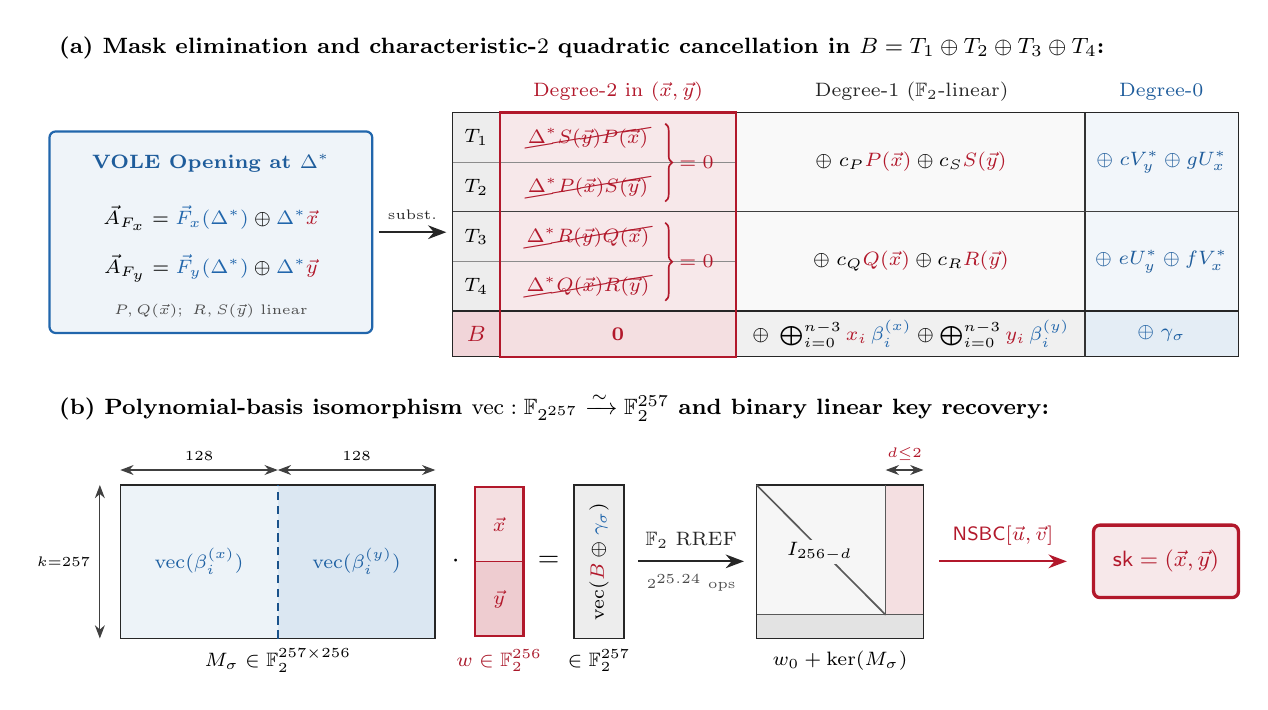
\begin{tikzpicture}[
    >=Stealth,
    font=\footnotesize,
    matborder/.style={semithick, draw=black!85},
    dimarrow/.style={<->, >=Stealth, thin, draw=black!75}
]
    % =========================================================================
    % PANEL (a): Mask Elimination & Pairwise Quadratic Cancellation in B
    % =========================================================================
    \node[anchor=west, font=\footnotesize\bfseries] at (0.00, 6.78) {(a) Mask elimination and characteristic-$2$ quadratic cancellation in $B = T_1 \oplus T_2 \oplus T_3 \oplus T_4$:};

    % Left Single Clean Box: Opened VOLE Substitution (x: 0.00..4.10, y: 3.16..5.72)
    \fill[accentblue!7, rounded corners=0.8mm] (0.00, 3.16) rectangle (4.10, 5.72);
    \draw[thick, accentblue, rounded corners=0.8mm] (0.00, 3.16) rectangle (4.10, 5.72);
    \node[font=\scriptsize\bfseries, text=accentblue!90!black] at (2.05, 5.32) {VOLE Opening at $\Delta^*$};
    \node[font=\scriptsize] at (2.05, 4.62) {$\vec{A}_{F_x} = {\color{accentblue}\vec{F}_x(\Delta^*)} \oplus {\color{accentblue}\Delta^*}{\color{accentred}\vec{x}}$};
    \node[font=\scriptsize] at (2.05, 3.98) {$\vec{A}_{F_y} = {\color{accentblue}\vec{F}_y(\Delta^*)} \oplus {\color{accentblue}\Delta^*}{\color{accentred}\vec{y}}$};
    \node[font=\tiny, text=black!70] at (2.05, 3.44) {$P, Q(\vec{x});\; R, S(\vec{y})$ linear};

    % Substitution Arrow
    \draw[->, thick, black!85] (4.18, 4.44) -- node[above=1pt, font=\tiny] {subst.} (5.04, 4.44);

    % Right Structured Decomposition Table (x: 5.12..15.10, y: 2.86..5.96)
    \node[font=\scriptsize, text=accentred] at (7.22, 6.22) {Degree-2 in $(\vec{x},\vec{y})$};
    \node[font=\scriptsize, text=black!85] at (10.95, 6.22) {Degree-1 ($\Ftwo$-linear)};
    \node[font=\scriptsize, text=accentblue!90!black] at (14.12, 6.22) {Degree-0};

    % Column backgrounds for T_1..T_4 (y: 3.44..5.96)
    \fill[gray!14]      (5.12, 3.44) rectangle (5.72, 5.96);
    \fill[accentred!10] (5.72, 3.44) rectangle (8.72, 5.96);
    \fill[gray!5]       (8.72, 3.44) rectangle (13.15, 5.96);
    \fill[accentblue!6] (13.15, 3.44) rectangle (15.10, 5.96);

    % Sum row backgrounds (y: 2.86..3.44)
    \fill[accentred!18] (5.12, 2.86) rectangle (5.72, 3.44);
    \fill[accentred!14] (5.72, 2.86) rectangle (8.72, 3.44);
    \fill[gray!12]      (8.72, 2.86) rectangle (13.15, 3.44);
    \fill[accentblue!12](13.15, 2.86) rectangle (15.10, 3.44);

    % Grid lines
    \draw[matborder] (5.12, 2.86) rectangle (15.10, 5.96);
    \draw[semithick, black!80] (5.72, 2.86) -- (5.72, 5.96)
                               (8.72, 2.86) -- (8.72, 5.96)
                               (13.15, 2.86) -- (13.15, 5.96);
    \draw[thin, black!45] (5.12, 5.33) -- (8.72, 5.33)
                          (5.12, 4.07) -- (8.72, 4.07);
    \draw[thin, black!75] (5.12, 4.70) -- (15.10, 4.70);
    \draw[thick, black!85] (5.12, 3.44) -- (15.10, 3.44);
    \draw[thick, accentred] (5.72, 2.86) rectangle (8.72, 5.96);

    % Row labels
    \node[font=\scriptsize\bfseries] at (5.42, 5.64) {$T_1$};
    \node[font=\scriptsize\bfseries] at (5.42, 5.01) {$T_2$};
    \node[font=\scriptsize\bfseries] at (5.42, 4.38) {$T_3$};
    \node[font=\scriptsize\bfseries] at (5.42, 3.75) {$T_4$};
    \node[font=\footnotesize\bfseries, text=accentred] at (5.42, 3.15) {$B$};

    % Col 1: Cancelled Quadratic Terms
    \node[font=\scriptsize, text=accentred] at (6.84, 5.64) {$\cancel{\Delta^* S(\vec{y}) P(\vec{x})}$};
    \node[font=\scriptsize, text=accentred] at (6.84, 5.01) {$\cancel{\Delta^* P(\vec{x}) S(\vec{y})}$};
    \draw[decorate, decoration={brace, amplitude=2.5pt}, semithick, accentred] (7.82, 5.82) -- node[right=1.5pt, font=\scriptsize, text=accentred] {$=0$} (7.82, 4.83);

    \node[font=\scriptsize, text=accentred] at (6.84, 4.38) {$\cancel{\Delta^* R(\vec{y}) Q(\vec{x})}$};
    \node[font=\scriptsize, text=accentred] at (6.84, 3.75) {$\cancel{\Delta^* Q(\vec{x}) R(\vec{y})}$};
    \draw[decorate, decoration={brace, amplitude=2.5pt}, semithick, accentred] (7.82, 4.56) -- node[right=1.5pt, font=\scriptsize, text=accentred] {$=0$} (7.82, 3.57);

    \node[font=\scriptsize\bfseries, text=accentred] at (7.22, 3.15) {$\mathbf{0}$};

    % Col 2: Clean Pairwise-Grouped Surviving F_2-Linear Terms
    \node[font=\scriptsize] at (10.94, 5.33) {$\oplus\; c_P {\color{accentred}P(\vec{x})} \oplus c_S {\color{accentred}S(\vec{y})}$};
    \node[font=\scriptsize] at (10.94, 4.07) {$\oplus\; c_Q {\color{accentred}Q(\vec{x})} \oplus c_R {\color{accentred}R(\vec{y})}$};
    \node[font=\scriptsize] at (10.94, 3.15) {$\oplus\;\bigoplus_{i=0}^{n-3} {\color{accentred}x_i}\,{\color{accentblue}\beta_i^{(x)}} \oplus \bigoplus_{i=0}^{n-3} {\color{accentred}y_i}\,{\color{accentblue}\beta_i^{(y)}}$};

    % Col 3: Clean Pairwise-Grouped Public Constant Terms
    \node[font=\scriptsize, text=accentblue!90!black] at (14.12, 5.33) {$\oplus\; c V_y^* \oplus g U_x^*$};
    \node[font=\scriptsize, text=accentblue!90!black] at (14.12, 4.07) {$\oplus\; e U_y^* \oplus f V_x^*$};
    \node[font=\scriptsize\bfseries, text=accentblue!95!black] at (14.12, 3.15) {$\oplus\; \gamma_\sigma$};

    % =========================================================================
    % PANEL (b): Binary Matrix Equation & Recovery Pipeline
    % =========================================================================
    \node[anchor=west, font=\footnotesize\bfseries] at (0.00, 2.22) {(b) Polynomial-basis isomorphism $\vecF : \FtwoN \xrightarrow{\sim} \Ftwo^{257}$ and binary linear key recovery:};

    \begin{scope}[yshift=-0.22cm]
    % Matrix M_\sigma (x: 0.90..4.90, y: -0.50..1.45)
    \fill[accentblue!8]  (0.90, -0.50) rectangle (2.90, 1.45);
    \fill[accentblue!16] (2.90, -0.50) rectangle (4.90, 1.45);
    \draw[matborder] (0.90, -0.50) rectangle (4.90, 1.45);
    \draw[semithick, accentblue!80!black, densely dashed] (2.90, -0.50) -- (2.90, 1.45);
    \draw[dimarrow] (0.64, -0.50) -- node[left, font=\tiny] {$k{=}257$} (0.64, 1.45);
    \draw[dimarrow] (0.90, 1.64) -- node[above, font=\tiny] {$128$} (2.90, 1.64);
    \draw[dimarrow] (2.90, 1.64) -- node[above, font=\tiny] {$128$} (4.90, 1.64);
    \node[font=\scriptsize, text=accentblue!95!black] at (1.90, 0.48) {$\vecF(\beta_i^{(x)})$};
    \node[font=\scriptsize, text=accentblue!95!black] at (3.90, 0.48) {$\vecF(\beta_i^{(y)})$};
    \node[font=\scriptsize] at (2.90, -0.78) {$M_\sigma \in \Ftwo^{257 \times 256}$};

    \node[font=\normalsize] at (5.16, 0.48) {$\cdot$};

    % Secret Vector w = (x || y)^T (x: 5.40..6.02, y: -0.47..1.42)
    \fill[accentred!14] (5.40, 0.48) rectangle (6.02, 1.42);
    \fill[accentred!22] (5.40, -0.47) rectangle (6.02, 0.48);
    \draw[thick, accentred] (5.40, -0.47) rectangle (6.02, 1.42);
    \draw[semithick, accentred] (5.40, 0.48) -- (6.02, 0.48);
    \node[font=\scriptsize\bfseries, text=accentred] at (5.71, 0.95) {$\vec{x}$};
    \node[font=\scriptsize\bfseries, text=accentred] at (5.71, 0.00) {$\vec{y}$};
    \node[font=\scriptsize, text=accentred!95!black] at (5.71, -0.78) {$w \in \Ftwo^{256}$};

    \node[font=\normalsize] at (6.34, 0.48) {$=$};

    % RHS Vector vec(B \oplus \gamma_\sigma) (x: 6.66..7.30, y: -0.50..1.45)
    \fill[gray!14] (6.66, -0.50) rectangle (7.30, 1.45);
    \draw[matborder] (6.66, -0.50) rectangle (7.30, 1.45);
    \node[font=\scriptsize, rotate=90] at (6.98, 0.48) {$\vecF({\color{accentred}B} \oplus {\color{accentblue}\gamma_\sigma})$};
    \node[font=\scriptsize] at (6.98, -0.78) {$\in \Ftwo^{257}$};

    % RREF Arrow
    \draw[->, thick, black!85] (7.48, 0.48) -- node[above=1pt, font=\scriptsize] {$\Ftwo$ RREF} node[below=1pt, font=\tiny, text=black!70] {$2^{25.24}$ ops} (8.82, 0.48);

    % Echelon Matrix [I_{256-d} | * ; 0] (x: 8.98..11.10, y: -0.50..1.45)
    \fill[gray!7]       (8.98, -0.20) rectangle (10.62, 1.45);
    \fill[accentred!14] (10.62, -0.20) rectangle (11.10, 1.45);
    \fill[gray!22]      (8.98, -0.50) rectangle (11.10, -0.20);
    \draw[matborder] (8.98, -0.50) rectangle (11.10, 1.45);
    \draw[thin, black!65] (8.98, -0.20) -- (11.10, -0.20)
                          (10.62, -0.20) -- (10.62, 1.45);
    \draw[semithick, black!65] (8.98, 1.45) -- (10.62, -0.20);
    \node[font=\scriptsize, fill=gray!7, inner sep=1pt] at (9.78, 0.60) {$I_{256-d}$};
    \draw[dimarrow] (10.62, 1.64) -- node[above, font=\tiny, text=accentred] {$d{\le}2$} (11.10, 1.64);
    \node[font=\scriptsize] at (10.04, -0.78) {$w_0 + \ker(M_\sigma)$};

    % NSBC filter arrow
    \draw[->, thick, accentred] (11.30, 0.48) -- node[above=2pt, font=\scriptsize, text=accentred] {$\NSBC[\vec{u},\vec{v}]$} (12.92, 0.48);

    % Recovered Secret Key Box (x: 13.26..15.10, width 1.84cm)
    \fill[accentred!10, rounded corners=0.8mm] (13.26, 0.02) rectangle (15.10, 0.94);
    \draw[very thick, accentred, rounded corners=0.8mm] (13.26, 0.02) rectangle (15.10, 0.94);
    \node[font=\footnotesize\bfseries, text=accentred] at (14.18, 0.48) {$\sk = (\vec{x}, \vec{y})$};
    \end{scope}
\end{tikzpicture}
\caption{Visualisation of single-signature secret-key recovery (Lemma~\ref{thm:B-affine}, Theorem~\ref{thm:key-recovery}, and Algorithm~1). \textbf{(a)}~Substituting the public VOLE evaluations $\vec{A}_{F_x} = \vec{F}_x(\Delta^*) \oplus \Delta^*\vec{x}$ and $\vec{A}_{F_y} = \vec{F}_y(\Delta^*) \oplus \Delta^*\vec{y}$ (blue) into $B = T_1 \oplus T_2 \oplus T_3 \oplus T_4$ cancels every quadratic cross-term in $(\vec{x}, \vec{y})$ pairwise in characteristic~$2$, collapsing $B$ to a noiseless $\Ftwo$-affine functional. \textbf{(b)}~Expanding over the polynomial basis of $\FtwoN$ yields a $257 \times 256$ binary system $M_\sigma w = \vecF(B \oplus \gamma_\sigma)$ with kernel dimension $d \le 2$, uniquely solved via Gaussian elimination and the public $\NSBC$ test.}
\label{fig:attack-cancellation}
\end{figure}

\begin{figure}[t]
\centering
\small
\begin{tabular}{@{}p{0.97\textwidth}@{}}
\toprule
\textbf{Algorithm 1:} Single-Signature Secret-Key Recovery against $\SBCVOLE$ and $\SBCVOLEM$ \\
\midrule
\textbf{Input:} Public key $\pk = (\vec{u}, \vec{v}) \in (\Ftwok)^n \times (\Ftwok)^n$, message $\msg$, valid signature $\sigma$. \\
\textbf{Output:} Candidate witness set $\mathcal{W}_\sigma \subseteq \NSBC[\vec{u}, \vec{v}]$ containing $\sk = (\vec{x}, \vec{y})$. \\[2pt]
\textbf{1.} Run the public verification reconstruction (Section~\ref{subsec:verifier-reconstructs}) on $(\pk, \msg, \sigma)$ to obtain $\Delta^* \in \Ftwok$ and $\vec{F}_x(\Delta^*), \vec{F}_y(\Delta^*) \in (\Ftwok)^{n-2}$. \\
\textbf{2.} Compute $U_x^*, V_x^*, U_y^*, V_y^* \in \Ftwok$ via~\eqref{eq:UxVxUyVy} and $c_P, c_Q, c_R, c_S, \gamma_\sigma \in \Ftwok$ via~\eqref{eq:cPQRS}. \\
\textbf{3.} \textbf{for} $i = 0$ \textbf{to} $n - 3$ \textbf{do} \\
\hspace*{1.8em} Compute $\beta_i^{(x)} \leftarrow c_P u_i \oplus c_Q v_i$ and $\beta_i^{(y)} \leftarrow c_R u_i \oplus c_S v_i$ in $\Ftwok$. \\
\hspace*{1.8em} Set column $i$ of $M_\sigma$ to $\vecF(\beta_i^{(x)})$ and column $(n - 2 + i)$ of $M_\sigma$ to $\vecF(\beta_i^{(y)})$. \\
\textbf{4.} Solve the $k \times 2(n-2)$ binary linear system $M_\sigma w = \vecF(B \oplus \gamma_\sigma)$ over $\Ftwo$ via Gaussian elimination to obtain a particular solution $w_0$ and a basis of $\ker(M_\sigma)$, where $d = 2(n-2) - \rank(M_\sigma)$. \\
\textbf{5.} Return $\mathcal{W}_\sigma \leftarrow \big\{(\tilde{\vec{x}}, \tilde{\vec{y}}) : (\tilde{\vec{x}}, \tilde{\vec{y}})^\top \in w_0 + \ker(M_\sigma) \text{ and } ((\tilde{\vec{x}}, 1, 0), (\tilde{\vec{y}}, 0, 1)) \in \NSBC[\vec{u}, \vec{v}]\big\}$. \\
\bottomrule
\end{tabular}
\end{figure}

\begin{theorem}[Single-Signature Secret-Key Recovery]
\label{thm:key-recovery}
Let $(\pk, \sk)$ be any key pair of $\SBCVOLE$ or $\SBCVOLEM$ over $\Ftwok / \Ftwo$, and let $\sigma$ be any honestly generated signature on a message $\msg$ inducing a linear system~\eqref{eq:linear-system} of kernel dimension $d = 2(n-2) - \rank(M_\sigma)$. Then Algorithm~1 returns a non-empty witness set $\mathcal{W}_\sigma \subseteq \NSBC[\vec{u}, \vec{v}]$ of size at most $2^d$ that contains the signer's secret key $\sk = (\vec{x}, \vec{y})$, using (to leading order in Gaussian elimination)
\begin{equation}
\label{eq:cost-formula}
T(n, k) = \underbrace{4(n-2) k^2}_{\text{forming } \beta_i^{(x)}, \beta_i^{(y)}} + \underbrace{\frac{1}{3} k \big(2(n-2)\big)^2}_{\text{GF(2) elimination}} + \underbrace{2^d \big(4(n-2)k + 2k^2\big)}_{\NSBC \text{ candidate check}}
\end{equation}
elementary bit operations beyond a single signature verification.
\end{theorem}

\begin{proof}
Lemma~\ref{thm:B-affine} reduces the verification slope $B$ to a single scalar equation over $\Ftwok$ in the binary coordinates of $(\vec{x}, \vec{y}) \in \Ftwo^{n-2} \times \Ftwo^{n-2}$. Following the classical subfield-basis expansion (Weil restriction) used by Huth and Joux~\cite[Section~2.2]{HJ24} to expand~\eqref{eq:sbc} into $k$ bilinear equations over $\Ftwo$ in $2(n-2)$ binary unknowns---where the $\lambda = 128$-bit parameters $(k, n) = (257, 130)$ from collision resistance and prime-extension selection~\cite[Sections~2.2 and~4.1]{HJ24} satisfy $k = 257 > 2(n-2) = 256$---we apply the polynomial-basis isomorphism $\vecF : \Ftwok \xrightarrow{\sim} \Ftwo^k$ from~\eqref{eq:vec-linearity} to~\eqref{eq:B-closed}. Because scalar multiplication by $x_i, y_i \in \Ftwo$ commutes with $\vecF$, a single $\Ftwok$-affine equation decomposes into $k$ linear equations over $\Ftwo$ in the $2(n-2)$ secret bits, reducing the candidate space to a low-dimensional affine coset $w_0 + \ker(M_\sigma)$ that is filtered against~\eqref{eq:sbc}. We establish the theorem in three steps: (1) proving completeness of the binary linear reduction; (2) bounding the affine solution space and proving exactness of the $\NSBC$ filter; and (3) accounting for the bit-operation complexity.

\smallskip\noindent
\emph{Step 1: Completeness of the $\Ftwo$-linear reduction.}
Let $\sigma$ be an honestly generated signature under $\sk = (\vec{x}, \vec{y})$ with normalised witness $(\vec{x}', \vec{y}') = ((\vec{x}, 1, 0), (\vec{y}, 0, 1)) \in \NSBC[\vec{u}, \vec{v}]$. By Lemma~\ref{thm:B-affine}, the transmitted field element $B \in \Ftwok$ satisfies
\[
\bigoplus_{i=0}^{n-3} x_i \, \beta_i^{(x)} \oplus \bigoplus_{i=0}^{n-3} y_i \, \beta_i^{(y)} = B \oplus \gamma_\sigma \quad \text{in } \Ftwok.
\]
Applying $\vecF : \Ftwok \xrightarrow{\sim} \Ftwo^k$ to both sides and using the $\Ftwo$-linearity identity~\eqref{eq:vec-linearity} yields
\[
\bigoplus_{i=0}^{n-3} x_i \, \vecF(\beta_i^{(x)}) \oplus \bigoplus_{i=0}^{n-3} y_i \, \vecF(\beta_i^{(y)}) = \vecF(B \oplus \gamma_\sigma) \quad \text{in } \Ftwo^k.
\]
By definition of $M_\sigma$ in~\eqref{eq:M-sigma}, the left-hand side equals the matrix-vector product $M_\sigma w^*$ for the true secret key vector $w^* = (\vec{x}, \vec{y})^\top \in \Ftwo^{2(n-2)}$. Hence $M_\sigma w^* = \vecF(B \oplus \gamma_\sigma)$, so the linear system in Step~4 of Algorithm~1 is always consistent.

\smallskip\noindent
\emph{Step 2: Solution-space cardinality and $\NSBC$ candidate filtering.}
Since $M_\sigma w = \vecF(B \oplus \gamma_\sigma)$ is consistent and $\dim_{\Ftwo} \ker(M_\sigma) = 2(n-2) - \rank(M_\sigma) = d$, Gaussian elimination in Step~4 returns an affine solution space $w_0 + \ker(M_\sigma) \subseteq \Ftwo^{2(n-2)}$ of exact cardinality $2^d$ containing $w^*$. In Step~5, each candidate $(\tilde{\vec{x}}, \tilde{\vec{y}})^\top \in w_0 + \ker(M_\sigma)$ is tested against $((\tilde{\vec{x}}, 1, 0), (\tilde{\vec{y}}, 0, 1)) \in \NSBC[\vec{u}, \vec{v}]$. Because $(\vec{x}', \vec{y}') \in \NSBC[\vec{u}, \vec{v}]$, the true key $\sk = (\vec{x}, \vec{y})$ survives this filter, while every surviving candidate is by construction a valid normalised $\NSBC[\vec{u}, \vec{v}]$ witness. Thus $\sk \in \mathcal{W}_\sigma \subseteq \NSBC[\vec{u}, \vec{v}]$ and $1 \le |\mathcal{W}_\sigma| \le 2^d$.

\smallskip\noindent
\emph{Step 3: Bit-operation complexity.}
Beyond the public verification reconstruction of Section~\ref{subsec:verifier-reconstructs}, Step~3 evaluates $2(n-2)$ linear combinations $\beta_i^{(x)} = c_P u_i \oplus c_Q v_i$ and $\beta_i^{(y)} = c_R u_i \oplus c_S v_i$, requiring $4(n-2)$ multiplications in $\Ftwok$, or $4(n-2)k^2$ elementary bit operations under schoolbook polynomial arithmetic. Step~4 performs Gaussian elimination on $M_\sigma \in \Ftwo^{k \times 2(n-2)}$, requiring $\frac{1}{3} k (2(n-2))^2$ bit operations to leading order. Finally, Step~5 evaluates the four subfield-to-extension inner products $\vec{u}\cdot\tilde{\vec{x}}', \vec{v}\cdot\tilde{\vec{x}}', \vec{u}\cdot\tilde{\vec{y}}', \vec{v}\cdot\tilde{\vec{y}}'$ ($4(n-2)k$ bit operations via subset XORs) and two $\Ftwok$ multiplications ($2k^2$ bit operations) for each of the $2^d$ candidates, summing to~\eqref{eq:cost-formula}.
\end{proof}

\paragraph{Rank Deficiency and Concrete Complexity at $\lambda = 128$.}
At the $\lambda = 128$-bit parameters $(q, k, n) = (2, 257, 130)$, the unknown secret key has $2(n-2) = 256$ bits while~\eqref{eq:linear-system} provides $k = 257$ binary equations ($M_\sigma \in \Ftwo^{257 \times 256}$). A uniformly random $257 \times 256$ matrix over $\Ftwo$ has kernel dimension $d = 256 - \rank(M_\sigma)$ concentrated on $\{0, 1, 2\}$ ($\Pr[d = 0] \approx 0.578$, $\Pr[d = 1] \approx 0.385$, $\Pr[d = 2] \approx 0.037$), leaving at most $2^d \le 4$ affine candidates with probability above $99.9\%$; any false candidate fails the $257$-bit field identity~\eqref{eq:sbc} with probability $1 - 2^{-257}$, uniquely identifying $\sk$. Evaluating~\eqref{eq:cost-formula} at $(n, k) = (130, 257)$ and $d = 0$ gives $33{,}817{,}088 + 5{,}614{,}251 + 263{,}682 = 39{,}695{,}021 \approx 2^{25.24}$ bit operations ($9{,}258{,}690 \approx 2^{23.14}$ with Karatsuba multiplication, or $74{,}040{,}501 \approx 2^{26.14}$ if $U_x^*, V_x^*, U_y^*, V_y^*$, $c_P, c_Q, c_R, c_S$, and $\gamma_\sigma$ are also charged as full $k^2$ multiplications) and $257 \times 256 = 65{,}792$ bits ($8.0$~kB) of memory from $1$ signature. Neither $D$ nor $\tau$ enters~\eqref{eq:cost-formula}: every parameter set of both $\SBCVOLE$ and $\SBCVOLEM$ is broken with identical algebraic complexity, more than $101$ bits below the claimed $128$-bit security level.

\section{Conditional Entropy of \texorpdfstring{$B$}{B} and Security Proof Analysis}
\label{sec:proof-flaw}

Given that Huth and Joux provided an explicit EUF-CMA security reduction in Theorem~2 and Appendix~A of~\cite{HJ25}, we now pinpoint the exact step in their reduction where this leakage went undetected.

\subsection{The Witness-Free Simulator in Game~2}
In Section~5 of~\cite[p.~18, full version]{HJ25}, $\SBCVOLE$ is obtained by applying the Fiat--Shamir transform to the five-pass identification protocol of Section~\ref{sec:protocol}. In Appendix~A~\cite[pp.~33--35, full version]{HJ25}, the proof of EUF-CMA security proceeds via a hybrid game sequence from the real signing game (\textbf{Game~1}, which answers signing queries via the real oracle $\mathcal{O}(\sk, \pk)$) to a simulated signing game (\textbf{Game~2}, which replaces $\mathcal{O}(\sk, \pk)$ by a witness-free simulator $\mathcal{S}(\pk)$ that chooses random oracle outputs $h_0, h_1$ in advance).

To argue that $\mathcal{S}(\pk)$ reproduces the honest signature distribution without knowing $\sk$, the proof states verbatim~\cite[Appendix~A, p.~35, full version]{HJ25}:
\begin{quote}
\itshape
``The simulator then proceeds to derive the shares of $\vec{x}$ and $\vec{y}$ as in the original Signing algorithm, with the difference that $\vec{x}$ and the offset values $(\delta_{\vec{y}_j})_{j \in [\tau]}$ are picked at random. Therefore, $\vec{x}$ and the derived $\vec{y} = \sum_{i=0}^{N-1} \vec{y}_j^{\share{i}} + \delta_{\vec{y}_j}$ solve the $\SBC$ problem only with negligible probability. The simulator can then use the Verification algorithm to compute the expected values of $A, B, b$ and $(\delta_{z_j})_{j \in [\tau]^*}$. Using this simulator, the shares revealed in the signature are uniformly distributed under the condition that $\Phi(\Delta^*) = A + B\Delta^*$, i.e., they have the same distribution as the shares obtained from an honest signature execution. If the algorithms do not abort, the obtained signatures from $\mathcal{S}(\pk)$ and $\mathcal{O}(\sk, \pk)$ are therefore identically distributed.''
\end{quote}
From this claim, the proof concludes that $|\varepsilon_{\textup{Game 2}} - \varepsilon_{\textup{Game 1}}| \le Q^2 / 2^{2\lambda}$ (accounting only for $\salt$ collisions).

\subsection{Zero Conditional Entropy and Simulator Distinguisher}
Inspection of the Game~2 transition reveals both an operational contradiction and an algebraic error:

\paragraph{1. Verification Takes $B$ as Input Rather Than Output.}
In the verification algorithm~\cite[Section~5]{HJ25}, $B$, $b$, and $(\delta_{z_j})_{j \in [\tau]^*}$ are \emph{inputs} parsed from $\sigma$, not outputs computed by verification. Verification computes $\Phi(\Delta^*)$ from the opened VOLE evaluations and evaluates $A' \leftarrow \Phi(\Delta^*) \oplus B\Delta^*$, imposing only one scalar constraint $A' \oplus B\Delta^* = \Phi(\Delta^*)$ on the pair $(A', B)$ while leaving $B$ undetermined.

\paragraph{2. Zero Conditional Entropy of $B$ Given the Opened Transcript.}
In the predecessor CRYPTO 2024 MPCitH scheme~\cite{HJ24}, each virtual party $i \in [N]$ generated fresh random masks $R_A^{\share{i}}, R_B^{\share{i}} \in \Fqk$, and the unopened party's mask $R_B^{\share{i^*}}$ genuinely acted as a one-time pad on the transmitted offset $\delta_B$. When migrating to VOLEitH in~\cite{HJ25}, the per-party masks $R_A^{\share{i}}, R_B^{\share{i}}$ were removed under the implicit assumption that the unopened VOLE masks $\vec{A}_{F_x}, \vec{A}_{F_y}$ inside~\eqref{eq:B-def} would still randomise $B$. However, once the punctured keys and $(\delta_{\vec{y}_j})_{j \in [\tau]}$ are revealed in $\sigma$, the evaluations $\vec{F}_x(\Delta^*)$ and $\vec{F}_y(\Delta^*)$ are fixed, locking $\vec{A}_{F_x} = \vec{F}_x(\Delta^*) \oplus \Delta^*\vec{x}$ and $\vec{A}_{F_y} = \vec{F}_y(\Delta^*) \oplus \Delta^*\vec{y}$ deterministically to the witness. By Lemma~\ref{thm:B-affine}, in an honest signature under $\sk$, the coordinate vector $\vecF(B)$ is a deterministic point mass on $M_\sigma w \oplus \vecF(\gamma_\sigma)$:
\begin{equation}
\label{eq:zero-entropy}
H\Big(B \;\Big|\; \pk, \, \sk, \, \salt, \, K_{i^*_{\text{p}}}, \, K_{i^*_0, \dots, i^*_{\tau-1}}, \, (\delta_{\vec{y}_j})_{j \in [\tau]}, \, h_0, \, h_1\Big) = 0.
\end{equation}
More generally, any VOLEitH reduction that omits an explicit multiplication-gate mask must verify that transmitted polynomial coefficients retain full conditional entropy \emph{after} conditioning on the punctured VOLE evaluations, rather than inspecting mask entropy prior to opening.

\begin{theorem}[Refutation of HVZK Simulation and Game~2 Indistinguishability]
\label{prop:hvzk-refuted}
Let $\mathcal{D}$ be the polynomial-time distinguisher that, given $\pk = (\vec{u}, \vec{v})$ and one signature $\sigma$ (or interactive transcript), runs Algorithm~1 and outputs $1$ if and only if $\mathcal{W}_\sigma \neq \emptyset$. Then $\mathcal{D}$ outputs $1$ with probability~$1$ on honest signatures from $\mathcal{O}(\sk, \pk)$ (Game~1), whereas for any simulator $\mathcal{S}(\pk)$ running without knowledge of an $\NSBC[\vec{u}, \vec{v}]$ witness (Game~2),
\[
\big|\varepsilon_{\textup{Game 2}} - \varepsilon_{\textup{Game 1}}\big| \ge 1 - \varepsilon_{\SBC}
\]
after a single signing query ($q_s = 1$). In particular, at $(q, k, n) = (2, 257, 130)$, where $\pk \leftarrow \mathsf{KeyGen}(1^\lambda)$ plants $\sk \in \NSBC[\vec{u}, \vec{v}]$ so that $\mathbb{E}_{\pk}\big[|\NSBC[\vec{u}, \vec{v}]|\big] = 1 + (2^{2(n-2)} - 1)2^{-k} \approx 3/2$:
\begin{enumerate}[leftmargin=2em]
    \item If $\mathcal{S}(\pk)$ samples $B \xleftarrow{\$} \Ftwok$ uniformly and sets $A \leftarrow \Phi(\Delta^*) \oplus B\Delta^*$ (Strategy~$\mathcal{S}_1$), then $\vecF(B \oplus \gamma_\sigma) \notin \operatorname{im}(M_\sigma)$ with probability $1 - 2^{\rank(M_\sigma) - k} \ge 1/2$, and $\mathcal{W}_\sigma \neq \emptyset$ holds with probability at most $|\NSBC[\vec{u}, \vec{v}]| / 2^k$ ($\approx 3 \cdot 2^{-258} < 2^{-256}$ in expectation over $\mathsf{KeyGen}$).
    \item If $\mathcal{S}(\pk)$ samples a random dummy pair $(\tilde{\vec{x}}, \tilde{\vec{y}}) \xleftarrow{\$} \Ftwo^{n-2} \times \Ftwo^{n-2}$ as described in~\cite[p.~35, full version]{HJ25}, computes $B$ via~\eqref{eq:B-def}, and sets $A \leftarrow \Phi(\Delta^*) \oplus B\Delta^*$ (Strategy~$\mathcal{S}_2$), then $M_\sigma w = \vecF(B \oplus \gamma_\sigma)$ recovers $(\tilde{\vec{x}}, \tilde{\vec{y}})^\top \in w_0 + \ker(M_\sigma)$, which fails~\eqref{eq:sbc} with probability $1 - |\NSBC[\vec{u}, \vec{v}]| / 2^{2(n-2)}$, and $\mathcal{W}_\sigma \neq \emptyset$ holds with probability at most $2^d |\NSBC[\vec{u}, \vec{v}]| / 2^{2(n-2)}$ ($< 2^{-254}$ in expectation).
\end{enumerate}
\end{theorem}

\begin{proof}
The breakdown of the Game~1 $\to$ Game~2 transition stems from an incompatibility between zero conditional entropy and witness-free simulation. Because $B$ has zero conditional entropy given the opened transcript and $\sk$, Algorithm~1 functions as a deterministic algebraic extractor whenever $\vecF(B)$ lies in the image of $\NSBC[\vec{u}, \vec{v}]$ under the affine map $w \mapsto M_\sigma w \oplus \vecF(\gamma_\sigma)$. Consequently, any witness-free simulator $\mathcal{S}(\pk)$ that causes $\mathcal{D}$ to accept with probability $p$ immediately yields an algorithm that solves $\SBC[\vec{u}, \vec{v}]$ from $\pk$ alone with probability $p$. We first establish the general reduction bound $|\varepsilon_{\textup{Game 2}} - \varepsilon_{\textup{Game 1}}| \ge 1 - \varepsilon_{\SBC}$, and then derive the explicit acceptance probabilities of Strategies~$\mathcal{S}_1$ and~$\mathcal{S}_2$.

\smallskip\noindent
\emph{Step 1: General reduction to $\SBC[\vec{u}, \vec{v}]$.}
When $\sigma$ is generated by the real signing oracle $\mathcal{O}(\sk, \pk)$ in Game~1, Theorem~\ref{thm:key-recovery} guarantees $\sk \in \mathcal{W}_\sigma$, so $\mathcal{W}_\sigma \neq \emptyset$ and $\Pr[\mathcal{D}(\pk, \mathcal{O}(\sk, \pk)) = 1] = 1$. Suppose now that in Game~2 a witness-free simulator $\mathcal{S}(\pk)$ produces a transcript $\sigma_{\mathcal{S}} \leftarrow \mathcal{S}(\pk)$ satisfying $\Pr[\mathcal{D}(\pk, \sigma_{\mathcal{S}}) = 1] = p$. By Step~5 of Algorithm~1, every element of $\mathcal{W}_{\sigma_{\mathcal{S}}}$ is a valid solution in $\NSBC[\vec{u}, \vec{v}]$. Hence running $\mathcal{S}(\pk)$ once followed by Algorithm~1 solves the instance $\SBC[\vec{u}, \vec{v}]$ without access to $\sk$ with success probability $p \le \varepsilon_{\SBC}$, yielding $|\varepsilon_{\textup{Game 2}} - \varepsilon_{\textup{Game 1}}| = 1 - p \ge 1 - \varepsilon_{\SBC}$.

\smallskip\noindent
\emph{Step 2: Analysis of Strategy~$\mathcal{S}_1$ (uniform $B$) and Strategy~$\mathcal{S}_2$ (dummy witness).}
Under Strategy~$\mathcal{S}_1$, $B$ is chosen uniformly from $\Ftwok$, so $\vecF(B \oplus \gamma_\sigma)$ is uniform over $\Ftwo^k$. Since $\operatorname{im}(M_\sigma) \subseteq \Ftwo^k$ is a subspace of dimension $\rank(M_\sigma) \le 2(n-2) < k$, the linear system $M_\sigma w = \vecF(B \oplus \gamma_\sigma)$ has no solution with probability $1 - 2^{\rank(M_\sigma) - k} \ge 1 - 2^{2(n-2)-k} = 1/2$ at $(k, n) = (257, 130)$. Moreover, $\mathcal{W}_\sigma \neq \emptyset$ holds only if $\vecF(B \oplus \gamma_\sigma)$ falls into $\{M_\sigma w : w \in \NSBC[\vec{u}, \vec{v}]\}$, which has cardinality at most $|\NSBC[\vec{u}, \vec{v}]|$, bounding the acceptance probability by $|\NSBC[\vec{u}, \vec{v}]| / 2^k$; since $\mathsf{KeyGen}$ plants $\sk$ and each remaining pair satisfies~\eqref{eq:sbc} with probability $2^{-k}$, $\mathbb{E}_{\pk}[|\NSBC[\vec{u}, \vec{v}]|] = 1 + (2^{256}-1)2^{-257} \approx 3/2$, giving expectation $\approx 3 \cdot 2^{-258} < 2^{-256}$. Under Strategy~$\mathcal{S}_2$, Lemma~\ref{thm:B-affine} applies identically to the dummy vector $\tilde{w} = (\tilde{\vec{x}}, \tilde{\vec{y}})^\top \xleftarrow{\$} \Ftwo^{2(n-2)}$, so Step~4 of Algorithm~1 recovers $w_0 + \ker(M_\sigma) = \tilde{w} + \ker(M_\sigma)$. For any fixed coset offset $z \in \ker(M_\sigma)$, $\tilde{w} \oplus z$ is uniform over $\Ftwo^{2(n-2)}$ and lands in $\NSBC[\vec{u}, \vec{v}]$ with probability $|\NSBC[\vec{u}, \vec{v}]| / 2^{2(n-2)}$; union-bounding over the $2^d$ coset elements gives acceptance probability at most $2^d |\NSBC[\vec{u}, \vec{v}]| / 2^{2(n-2)}$ (and $\approx \frac{9}{4} \cdot 2^{-256} < 2^{-254}$ in expectation for uniform $M_\sigma$, where $\mathbb{E}[2^d] \approx 3/2$).
\end{proof}

\section{Protocol Repair via Correlated VOLE Masking}
\label{sec:repair}

Theorem~\ref{thm:key-recovery} and Theorem~\ref{prop:hvzk-refuted} show that both the key-recovery vulnerability and the Game~2 simulation failure stem from the zero conditional entropy of $B$ in~\eqref{eq:zero-entropy}. Restoring security therefore requires reinstating an independent degree-$1$ multiplication mask on $(A, B)$, following the standard VOLEitH multiplication-check paradigm of QuickSilver~\cite{YSWW21}, Baum et al.~\cite{BBDKORS23}, and FAEST~\cite{FAEST24} (and playing the VOLE analogue of the per-party masks $(R_A^{\share{i}}, R_B^{\share{i}})$ in~\cite{HJ24}).

\subsection{Insufficiency of Existing Leaf Shares}
None of the three existing leaf-expanded share families in $T_{\vec{x}_j}$ ($\vec{y}_j^{\share{\ell}} \in \Ftwo^{n-2}$, $z_j^{\share{\ell}} \in \Ftwok$, or $\com_j^{\share{\ell}} \in \{0,1\}^{2\lambda}$) can mask $B$ without adding fresh randomness:
\begin{enumerate}[leftmargin=2em]
    \item \textbf{Secret row $\vec{y}_j^{\share{\ell}}$:} Aligned via $\delta_{\vec{y}_j}$ to sum to the secret $\vec{y}$ itself.
    \item \textbf{Consistency pad $z_j^{\share{\ell}}$:} Already consumed by $b = z \oplus \vec{y} \cdot \vec{\mu}$ in~\eqref{eq:b-aj}; masking $B$ by $z$ (sending $\tilde{B} = B \oplus z$) leaves $\tilde{B} \oplus b = B \oplus \vec{y} \cdot \vec{\mu}$, which remains an unmasked $\Ftwo$-affine functional of $(\vec{x}, \vec{y})$.
    \item \textbf{Commitment row $\com_j^{\share{\ell}}$:} Completely revealed in $\SBCVOLE$ via $\com_j^{\share{1-b_{i,j}}_i} = X_j \oplus \com_j^{\share{b_{i,j}}_i}$, carrying zero conditional entropy in the verifier's view.
\end{enumerate}

\subsection{Correlated VOLE Masking Construction}
To integrate VOLE multiplication masking into $\SBCVOLE$ and $\SBCVOLEM$, we introduce one correlated field mask $\rho \in \Ftwok$ aligned across all $\tau$ trees via the same offset-and-$H_0$-binding mechanism that~\cite{HJ25} already uses for $z$ in~\eqref{eq:offsets} and~\eqref{eq:h0}:
\begin{enumerate}[leftmargin=2em]
    \item \textbf{Leaf Expansion:} Expand each leaf $\ell \in [2^D]$ of tree $T_{\vec{x}_j}$ ($j \in [\tau]$) into an additional share $\rho_j^{\share{\ell}} \in \Ftwok$ and fold via~\eqref{eq:folding-def} into $(\rho_j^{\share{0}_i}, \rho_j^{\share{1}_i})_{i \in [D]}$.
    \item \textbf{Global Mask and Offsets:} Set $\rho \leftarrow \rho_0^{\share{0}_0} \oplus \rho_0^{\share{1}_0} \in \Ftwok$ from tree $T_{\vec{x}_0}$, and for each $j \in [\tau]^*$ compute
    \[
    \delta_{\rho_j} \leftarrow \rho \oplus \rho_j^{\share{0}_0} \oplus \rho_j^{\share{1}_0} \in \Ftwok \qquad (\text{with } \delta_{\rho_0} := 0 \text{ omitted}).
    \]
    \item \textbf{Pre-Challenge Hash Binding:} Bind $(\delta_{\rho_j})_{j \in [\tau]^*}$ inside the first Fiat--Shamir hash:
    \begin{equation}
    \label{eq:h0-repaired}
    h_0 \leftarrow H_0\Big(\msg, h_{\com}, \salt, (\delta_{\vec{y}_j}, \delta_{z_j}, \delta_{\rho_j})_{j \in [\tau]}, (X_j)_{j \in [\tau]}\Big).
    \end{equation}
    \item \textbf{Masked Coefficients:} Compute $A_{F_\rho} \leftarrow \bigoplus_{j=0}^{\tau-1} \bigoplus_{i=jD}^{(j+1)D-1} \alpha_i \, \rho_j^{\share{0}_{i - jD}} \in \Ftwok$ and set
    \begin{equation}
    \label{eq:tilde-AB}
    \tilde{A} \leftarrow A \oplus A_{F_\rho} \in \Ftwok, \qquad \tilde{B} \leftarrow B \oplus \rho \in \Ftwok.
    \end{equation}
    Hash $(\tilde{A}, \tilde{B})$ in place of $(A, B)$ into $h_1$, and transmit $\tilde{B}$ and $(\delta_{\rho_j})_{j \in [\tau]^*}$ in $\sigma$.
    \item \textbf{Verification Unmasking:} The verifier reconstructs the opened mask VOLE evaluation
    \begin{equation}
    \label{eq:W-ver}
    F_\rho(\Delta^*) \leftarrow \bigoplus_{j=0}^{\tau-1} \bigoplus_{i=jD}^{(j+1)D-1} \alpha_i \left(\rho_j^{\share{b_{i-jD,j}}_{i-jD}} \oplus b_{i-jD,j} \, \delta_{\rho_j}\right) = A_{F_\rho} \oplus \Delta^* \rho,
    \end{equation}
    computes $\tilde{A}' \leftarrow \Phi(\Delta^*) \oplus F_\rho(\Delta^*) \oplus \tilde{B}\Delta^*$, and verifies that the recomputed digest $h'_1$ matches $h_1$.
\end{enumerate}

\subsection{Soundness Neutrality and Restored Simulation}

\begin{theorem}[Soundness Neutrality and Restored Simulation]
\label{prop:repair-security}
The repaired $\SBCVOLE$ and $\SBCVOLEM$ protocols satisfy:
\begin{enumerate}[leftmargin=2em]
    \item \textbf{Exact Soundness Preservation:} The five-pass identification protocol retains the exact soundness error bound $\varepsilon = \tau^2 2^{-k} + 2^{1 - \tau D}$~\cite[Theorem~1]{HJ25}.
    \item \textbf{Restored Game~2 Simulation:} There exists a polynomial-time witness-free simulator $\mathcal{S}_{\textup{repaired}}(\pk)$ in Game~2 whose output distribution on the masked verification transcript is indistinguishable from $\mathcal{O}(\sk, \pk)$ up to PRG and random-oracle collision bounds (orthogonal to commitment-binding~\cite{KLS25} and $\cGGM$ root-prefix reduction bounds~\cite{KX26,FR26}).
    \item \textbf{Multi-Signature Linear Security:} Across any $m \ge 1$ signatures under $\sk$, the joint linear system in $(\vec{x}, \vec{y})$ and the per-signature masks $(\rho^{(0)}, \dots, \rho^{(m-1)})$ maintains constant rank deficiency $2(n-2)$, leaking zero linear information about $(\vec{x}, \vec{y})$.
\end{enumerate}
\end{theorem}

\begin{proof}
Masking $B$ without disturbing the degree-$1$ verification check relies on lifting the folded shares of $\rho \in \Ftwok$ into the auxiliary VOLE evaluation $F_\rho(\Delta^*) = A_{F_\rho} \oplus \Delta^*\rho$. In the verifier's linear combination $\Phi(\Delta^*) \oplus F_\rho(\Delta^*) \oplus \tilde{B}\Delta^*$, the $\Delta^*\rho$ term cancels the shift in $\tilde{B} = B \oplus \rho$, translating the reconstructed constant term from $A$ to $\tilde{A} = A \oplus A_{F_\rho}$. We prove the three claims sequentially: (1) algebraic equivalence of the verification check at every challenge point $\Delta^*$; (2) conditional independence and uniformity of $\tilde{B}$ and $(\delta_{\rho_j})_{j \in [\tau]^*}$ given the punctured keys, which restores Game~2 simulation; and (3) rank-deficiency invariance across $m$ signatures.

\smallskip\noindent
\emph{Step 1: Exact soundness equivalence.}
When $(\delta_{\rho_j})_{j \in [\tau]^*}$ is bound in $h_0$ via~\eqref{eq:h0-repaired} before $(\alpha_m)_{m \in [\tau D]}$ are derived, the prover commits to a fixed sequence of tree masks $\rho_j = \rho_j^{\share{0}_0} \oplus \rho_j^{\share{1}_0} \oplus \delta_{\rho_j}$. Substituting~\eqref{eq:tilde-AB} and~\eqref{eq:W-ver} into the verifier's reconstructed constant $\tilde{A}'$ yields
\[
\tilde{A}' = \Phi(\Delta^*) \oplus (A_{F_\rho} \oplus \Delta^* \rho) \oplus (B \oplus \rho)\Delta^*
           = \big(\Phi(\Delta^*) \oplus B\Delta^*\big) \oplus A_{F_\rho}.
\]
Since $\tilde{A} = A \oplus A_{F_\rho}$, the equality $\tilde{A}' = \tilde{A}$ holds if and only if $\Phi(\Delta^*) \oplus B\Delta^* = A$. Hence the set of accepting second-round challenges $(i^*_j)_{j \in [\tau]}$ for any cheating prover is identical to that of the original protocol, preserving $\varepsilon = \tau^2 2^{-k} + 2^{1 - \tau D}$.

\smallskip\noindent
\emph{Step 2: Restored witness-free simulation.}
Conditioned on the punctured keys $(K_{i^*_{\text{p}}}, K_{i^*_0, \dots, i^*_{\tau-1}})$ and PRG security, the unopened leaf share $\rho_0^{\share{i^*_0}} \in \Ftwok$ in tree $T_{\vec{x}_0}$ is pseudorandom and appears in no opened branch share $\rho_0^{\share{b_{i,0}}_i}$. Thus $\rho = \rho_0^{\share{0}_0} \oplus \rho_0^{\share{1}_0}$ acts as an independent one-time pad on $\tilde{B} = B \oplus \rho$, while each unopened leaf share $\rho_j^{\share{i^*_j}}$ ($j \in [\tau]^*$) independently masks $\delta_{\rho_j} = \rho \oplus \rho_j^{\share{0}_0} \oplus \rho_j^{\share{1}_0}$. Consequently, a witness-free simulator $\mathcal{S}_{\textup{repaired}}(\pk)$ that samples $\tilde{B} \xleftarrow{\$} \Ftwok$ and $(\delta_{\rho_j})_{j \in [\tau]^*} \xleftarrow{\$} (\Ftwok)^{\tau-1}$ uniformly at random and sets $\tilde{A} \leftarrow \Phi(\Delta^*) \oplus F_\rho(\Delta^*) \oplus \tilde{B}\Delta^*$ produces transcripts whose distribution matches $\mathcal{O}(\sk, \pk)$ up to $\varepsilon_{\PRG}$ and random-oracle collision bounds.

\smallskip\noindent
\emph{Step 3: Multi-signature linear security.}
In signature $r \in [m]$, expanding $\tilde{B}^{(r)} = B^{(r)} \oplus \rho^{(r)}$ over $\Ftwo^k$ yields the $k$-row linear equation $M_{\sigma^{(r)}} w \oplus \vecF(\rho^{(r)}) = \vecF(\tilde{B}^{(r)} \oplus \gamma_{\sigma^{(r)}})$. Stacking $m$ signatures produces an $mk \times (2(n-2) + mk)$ binary system whose matrix is $\big[\, M \;\big|\; I_{mk} \,\big]$, which has full row rank $mk$ and constant kernel dimension $2(n-2)$ for every $m \ge 1$.
\end{proof}

\paragraph{Necessity of Pre-Challenge Hash Binding.}
Including $(\delta_{\rho_j})_{j \in [\tau]^*}$ inside $H_0$ in~\eqref{eq:h0-repaired} is essential for soundness. Because $\delta_{\rho_j}$ enters $F_\rho(\Delta^*)$ linearly as $\bigoplus_{j=1}^{\tau-1} \Delta^*_j \delta_{\rho_j}$, omitting $(\delta_{\rho_j})_{j \in [\tau]^*}$ from $H_0$ would let a keyless attacker commit to dummy vectors $(\tilde{\vec{x}}, \tilde{\vec{y}})$, obtain $(\Delta^*_j)_{j \in [\tau]}$, and solve a linear equation in $\Ftwok$ for $\delta_{\rho_j}$ whenever $\Delta^*_j \neq 0$ for some $j \ge 1$ (probability $1 - 2^{-D(\tau-1)}$) to force $\tilde{A}' = \tilde{A}$.

\subsection{Signature-Size Overhead and Post-Repair Standing}
Replacing $B$ by $\tilde{B}$ adds zero bits, while appending $(\delta_{\rho_1}, \dots, \delta_{\rho_{\tau-1}}) \in (\Ftwok)^{\tau-1}$ adds $\tau - 1$ elements of $\Ftwok$. Under the bit-packing rule of~\cite{HJ25} for $k = 257$ (each $\FtwoN$ element occupies $32$ bytes plus $1$ bit packed $8$-per-byte across all transmitted $\FtwoN$ elements, increasing the packed element count from $\tau + 1$ to $2\tau$), the exact byte overhead is
\begin{equation}
\label{eq:delta-bytes}
\Delta |\sigma|(\tau) = 32(\tau - 1) + \left\lceil \frac{2\tau}{8} \right\rceil - \left\lceil \frac{\tau + 1}{8} \right\rceil \quad \text{bytes}.
\end{equation}

\begin{table}[t]
\centering
\caption{Signature sizes before and after the correlated VOLE-masking repair at $\lambda = 128$ ($q = 2, k = 257, n = 130$).}
\label{tab:repair-sizes}
\small
\setlength{\tabcolsep}{4.5pt}
\begin{tabular}{@{}ccrrrrrrr@{}}
\toprule
\multicolumn{2}{c}{\textbf{Params}} & \multicolumn{3}{c}{\textbf{Basic Scheme $\SBCVOLE$}} & \multicolumn{3}{c}{\textbf{MinMax Scheme $\SBCVOLEM$}} & \textbf{Added} \\
\cmidrule(lr){1-2} \cmidrule(lr){3-5} \cmidrule(lr){6-8}
$D$ & $\tau$ & Original & Repaired & Overhead & Original & Repaired & Overhead & Offsets \\
\midrule
$9$  & $15$ & $3{,}458$~B & $3{,}908$~B & $+13.0\%$ & $2{,}978$~B & $3{,}428$~B & $+15.1\%$ & $14$ \\
$10$ & $13$ & $3{,}218$~B & $3{,}604$~B & $+12.0\%$ & $2{,}802$~B & $3{,}188$~B & $+13.8\%$ & $12$ \\
$11$ & $12$ & $3{,}170$~B & $3{,}523$~B & $+11.1\%$ & $2{,}786$~B & $3{,}139$~B & $+12.7\%$ & $11$ \\
$12$ & $11$ & $3{,}090$~B & $3{,}411$~B & $+10.4\%$ & $2{,}738$~B & $3{,}059$~B & $+11.7\%$ & $10$ \\
$\mathbf{13}$ & $\mathbf{10}$ & $\mathbf{2{,}978}$~\textbf{B} & $\mathbf{3{,}267}$~\textbf{B} & $\mathbf{+9.7\%}$ & $\mathbf{2{,}658}$~\textbf{B} & $\mathbf{2{,}947}$~\textbf{B} & $\mathbf{+10.9\%}$ & $\mathbf{9}$ \\
$15$ & $9$  & $2{,}978$~B & $3{,}235$~B & $+8.6\%$  & $2{,}690$~B & $2{,}947$~B & $+9.6\%$  & $8$ \\
\bottomrule
\end{tabular}
\end{table}

Table~\ref{tab:repair-sizes} lists the resulting sizes across all six published $(D, \tau)$ pairs. Because $\Delta|\sigma|(\tau)$ grows with $\tau - 1$, $(D, \tau) = (15, 9)$ ($3{,}235$~B, $\approx 5.1$~ms signing and verification~\cite{HJ25}) overtakes the headline $(13, 10)$ set ($3{,}267$~B, $+289$~B or $+9.7\%$, $\approx 2.2$~ms) as the smallest repaired $\SBCVOLE$ configuration. At $3{,}235$--$3{,}267$~B, repaired $\SBCVOLE$ exceeds Dual-SDitH ($2{,}813$--$2{,}851$~B)~\cite{BFGNR24} and the smallest VOLEitH-MQ instantiation ($3.1$--$3.6$~kB)~\cite{Bui24}, confirming that the sub-$3$~kB headline size of $\SBCVOLE$ depended on omitting a mandatory multiplication mask. Even so, repaired $\SBCVOLE$ still saves $499$--$531$~bytes and roughly $90\%$ runtime over CRYPTO 2024 $\SBC$ ($3{,}766$~B)~\cite{HJ24}, and remains more compact than VOLEitH-PKP ($3{,}686$~B)~\cite{BBGK24}, FAEST-EM v2 ($3{,}906$~B)~\cite{FAEST24}, ReSolveD ($3{,}916$~B)~\cite{CLYYYZ24}, and FAEST v2 ($4{,}506$~B)~\cite{FAEST24} while keeping a $48$-byte public key. Although repaired $\SBCVOLEM$ reaches $2{,}947$~B at both $(13, 10)$ and $(15, 9)$, our $\rho$-masking repair addresses only the algebraic verification layer and does not harden the implicit MinMax commitment against~\cite{KLS25}.

\section{Experimental Verification}
\label{sec:experiments}

We implemented Algorithm~1 and evaluated single-signature secret-key recovery across all published parameter sets of $\SBCVOLE$ and $\SBCVOLEM$~\cite{HJ25}.

First, at $(q, k, n) = (2, 257, 130)$, we verified that the second difference $B(w_1) \oplus B(w_2) \oplus B(w_1 \oplus w_2) \oplus B(0)$ vanished across $200 / 200$ random trials, and that the closed-form identity~\eqref{eq:B-closed}--\eqref{eq:cPQRS} matched the four-term formula~\eqref{eq:B-def} with zero mismatches under both padding conventions ($\eta \in \{0, 1\}$).

Second, we ran Algorithm~1 end-to-end across all six published $(D, \tau)$ parameter sets and both variants ($\SBCVOLE$ and $\SBCVOLEM$), testing $100$ independent random key pairs per configuration ($1{,}200$ instances in total). Given only $\pk$ and a single valid signature $\sigma$, the solver forms and reduces $M_\sigma \in \Ftwo^{257 \times 256}$, recovers $\sk$, and produces a valid signature on a fresh message.

\begin{table}[t]
\centering
\caption{Single-signature key recovery and kernel-dimension distribution of $M_\sigma \in \Ftwo^{257 \times 256}$ across $1{,}200$ random instances ($100$ keys per cell).}
\label{tab:sweep-results}
\small
\setlength{\tabcolsep}{4pt}
\begin{tabular}{@{}ccrrrrrcrrrrr@{}}
\toprule
\multicolumn{2}{c}{\textbf{Params}} & \multicolumn{5}{c}{\textbf{Basic Scheme $\SBCVOLE$}} & & \multicolumn{5}{c}{\textbf{MinMax Scheme $\SBCVOLEM$}} \\
\cmidrule(lr){1-2} \cmidrule(lr){3-7} \cmidrule(lr){9-13}
$D$ & $\tau$ & Recov. & $d=0$ & $d=1$ & $d=2$ & Mean $d$ & & Recov. & $d=0$ & $d=1$ & $d=2$ & Mean $d$ \\
\midrule
$9$  & $15$ & $100/100$ & $56$ & $41$ & $3$ & $0.470$ & & $100/100$ & $51$ & $46$ & $3$ & $0.520$ \\
$10$ & $13$ & $100/100$ & $63$ & $33$ & $4$ & $0.410$ & & $100/100$ & $59$ & $37$ & $4$ & $0.450$ \\
$11$ & $12$ & $100/100$ & $58$ & $36$ & $6$ & $0.480$ & & $100/100$ & $62$ & $35$ & $3$ & $0.410$ \\
$12$ & $11$ & $100/100$ & $56$ & $41$ & $3$ & $0.470$ & & $100/100$ & $57$ & $40$ & $3$ & $0.460$ \\
$13$ & $10$ & $100/100$ & $54$ & $39$ & $7$ & $0.530$ & & $100/100$ & $59$ & $41$ & $0$ & $0.410$ \\
$15$ & $9$  & $100/100$ & $60$ & $38$ & $2$ & $0.420$ & & $100/100$ & $48$ & $47$ & $5$ & $0.570$ \\
\midrule
\multicolumn{2}{@{}l}{\textbf{Pooled}} & $\mathbf{600/600}$ & $\mathbf{347}$ & $\mathbf{228}$ & $\mathbf{25}$ & $\mathbf{0.463}$ & & $\mathbf{600/600}$ & $\mathbf{336}$ & $\mathbf{246}$ & $\mathbf{18}$ & $\mathbf{0.470}$ \\
\bottomrule
\end{tabular}
\end{table}

As reported in Table~\ref{tab:sweep-results}, Algorithm~1 recovered the exact $256$-bit secret key on $1{,}200 / 1{,}200$ ($100\%$) of tested instances, producing valid signatures on fresh messages in every case, while all negative controls (bit-flipped key, modified message, and replayed signature) were rejected ($0 / 51$). Pooled kernel dimensions were $\{d=0: 683, \, d=1: 474, \, d=2: 43\}$ ($\bar{d} = 0.467$, $d_{\max} = 2$), matching the theoretical distribution of a uniform $257 \times 256$ binary matrix, and single-core execution required $0.06$~s per signature.

\section{Conclusion}
\label{sec:conclusion}
This work demonstrates that the $2^{128}$ algebraic hardness of the Subfield Bilinear Collision problem does not prevent passive single-signature key recovery when its VOLEitH verification polynomial omits an independent multiplication mask. Once punctured VOLE evaluations are opened during verification, substituting the resulting affine mask relations into the unmasked slope $B$ cancels all quadratic witness cross-terms in characteristic~$2$ (and vanishes on every honest witness in odd characteristic $q > 2$), exposing the $256$-bit secret key of both $\SBCVOLE$ and $\SBCVOLEM$ in $2^{25.24}$ bit operations. Beyond repairing $\SBCVOLE$ via a correlated VOLE field mask at a $+8.6\%$--$15.1\%$ size overhead, our analysis illustrates a general verification principle for VOLE-in-the-Head security proofs: zero-knowledge simulators cannot treat polynomial verification coefficients as conditionally uniform without verifying positive conditional entropy \emph{after} conditioning on the opened VOLE evaluations.

\paragraph{Use of AI.}
The cryptanalytic results and artifacts were initially developed through an autonomous agent system powered by a MiniMax internal model. We validated the key technical claims and refined the presentation of the manuscript.

\begin{thebibliography}{99}

\bibitem{AGHHJY23}
C.~Aguilar-Melchor, N.~Gama, J.~Howe, A.~H\"{u}lsing, D.~Joseph, and D.~Yue,
``The return of the SDitH,'' in \emph{Advances in Cryptology -- EUROCRYPT 2023}, Part~V, LNCS, vol.~14008, pp.~564--596, Springer, 2023.

\bibitem{FAEST24}
C.~Baum, W.~Beullens, L.~Braun, C.~Delpech de Saint Guilhem, M.~Kloo\ss, C.~Majenz, S.~Mukherjee, E.~Orsini, S.~Ramacher, C.~Rechberger, L.~Roy, and P.~Scholl,
``FAEST v2: Algorithm Specifications,'' Version~2.0, NIST Post-Quantum Cryptography Additional Digital Signatures Round~2 Submission, 2025. Available at \url{https://faest.info/faest-spec-v2.0.pdf}.

\bibitem{BBDKORS23}
C.~Baum, L.~Braun, C.~Delpech de Saint Guilhem, M.~Kloo\ss, E.~Orsini, L.~Roy, and P.~Scholl,
``Publicly verifiable zero-knowledge and post-quantum signatures from VOLE-in-the-head,'' in \emph{Advances in Cryptology -- CRYPTO 2023}, Part~V, LNCS, vol.~14085, pp.~581--615, Springer, 2023. (Full version: IACR ePrint 2023/996.)

\bibitem{BBGK24}
S.~Bettaieb, L.~Bidoux, P.~Gaborit, and M.~Kulkarni,
``Modelings for generic PoK and applications: Shorter SD and PKP based signatures,'' Cryptology ePrint Archive, Paper 2024/1668, 2024.

\bibitem{BFGNR24}
L.~Bidoux, T.~Feneuil, P.~Gaborit, R.~Neveu, and M.~Rivain,
``Dual support decomposition in the head: Shorter signatures from rank SD and MinRank,'' in \emph{Advances in Cryptology -- ASIACRYPT 2024}, Part~II, LNCS, vol.~15485, pp.~38--69, Springer, 2024.

\bibitem{BN26}
P.~Briaud and R.~Neveu,
``Cryptanalysis of the Subfield Bilinear Collision Problem,'' \emph{IACR Communications in Cryptology}, vol.~3, no.~3, 2026, doi:10.62056/a0l2ip10. (Preprint: IACR ePrint 2026/916.)

\bibitem{Bui24}
D.~Bui,
``Shorter VOLEitH signature from multivariate quadratic,'' Cryptology ePrint Archive, Paper 2024/465, 2024. (Revised version published as ``Efficient multi-instance vector commitment and application to post-quantum signatures'' in \emph{Information Security and Privacy -- ACISP 2025}, Part~II, LNCS, vol.~15659, pp.~23--41, Springer, 2025.)

\bibitem{CLYYYZ24}
H.~Cui, H.~Liu, D.~Yan, K.~Yang, Y.~Yu, and K.~Zhang,
``ReSolveD: Shorter signatures from regular syndrome decoding and VOLE-in-the-head,'' in \emph{Public-Key Cryptography -- PKC 2024}, Part~I, LNCS, vol.~14601, pp.~229--258, Springer, 2024.

\bibitem{FR26}
T.~Feneuil and M.~Rivain,
``On the security of MPC-in-the-head signatures with correlated GGM trees,'' Cryptology ePrint Archive, Paper 2026/615, 2026.

\bibitem{FS86}
A.~Fiat and A.~Shamir,
``How to prove yourself: Practical solutions to identification and signature problems,'' in \emph{Advances in Cryptology -- CRYPTO~'86}, LNCS, vol.~263, pp.~186--194, Springer, 1987.

\bibitem{GGM86}
O.~Goldreich, S.~Goldwasser, and S.~Micali,
``How to construct random functions,'' \emph{Journal of the ACM}, vol.~33, no.~4, pp.~792--807, 1986.

\bibitem{GYW23}
X.~Guo, K.~Yang, X.~Wang, W.~Zhang, X.~Xie, J.~Zhang, and Z.~Liu,
``Half-tree: Halving the cost of tree expansion in COT and DPF,'' in \emph{Advances in Cryptology -- EUROCRYPT 2023}, Part~I, LNCS, vol.~14004, pp.~330--362, Springer, 2023.

\bibitem{HJ24}
J.~Huth and A.~Joux,
``MPC in the head using the subfield bilinear collision problem,'' in \emph{Advances in Cryptology -- CRYPTO 2024}, Part~I, LNCS, vol.~14920, pp.~39--70, Springer, 2024. (Full version: IACR ePrint 2023/1685.)

\bibitem{HJ25}
J.~Huth and A.~Joux,
``VOLE-in-the-Head Signatures from Subfield Bilinear Collisions,'' in \emph{Advances in Cryptology -- ASIACRYPT 2025}, Part~IV, LNCS, vol.~16248, pp.~3--34, Springer, 2025. (Full version: IACR ePrint 2024/1537.)

\bibitem{IKOS07}
Y.~Ishai, E.~Kushilevitz, R.~Ostrovsky, and A.~Sahai,
``Zero-knowledge from secure multiparty computation,'' in \emph{Proceedings of the 39th Annual ACM Symposium on Theory of Computing (STOC 2007)}, pp.~21--30, ACM, 2007.

\bibitem{JP24}
A.~Joux and C.~Pierrot,
``Algorithmic aspects of elliptic bases in finite field discrete logarithm algorithms,'' \emph{Advances in Mathematics of Communications}, vol.~18, no.~5, pp.~1266--1302, 2024.

\bibitem{KLS25}
S.~Kim, B.~Lee, and M.~Son,
``Shorter VOLE-in-the-Head-based Signatures from Vector Semi-Commitment,'' Cryptology ePrint Archive, Paper 2025/1077, 2025. (Also in \emph{Proceedings of the 2026 ACM SIGSAC Conference on Computer and Communications Security (CCS 2026)}.)

\bibitem{KX26}
H.~Kosuge and K.~Xagawa,
``New security proofs of TC-in-the-head signatures in the quantum random oracle model,'' \emph{IACR Communications in Cryptology}, vol.~3, no.~3, 2026, doi:10.62056/akmpxruc2.

\bibitem{Roy22}
L.~Roy,
``SoftSpokenOT: Quieter OT extension from small-field silent VOLE in the minicrypt model,'' in \emph{Advances in Cryptology -- CRYPTO 2022}, Part~I, LNCS, vol.~13507, pp.~657--687, Springer, 2022.

\bibitem{YSWW21}
K.~Yang, P.~Sarkar, C.~Weng, and X.~Wang,
``QuickSilver: Efficient and affordable zero-knowledge proofs for circuits and polynomials over any field,'' in \emph{Proceedings of the 2021 ACM SIGSAC Conference on Computer and Communications Security (CCS 2021)}, pp.~2986--3001, ACM, 2021. (Full version: IACR ePrint 2021/076.)

\end{thebibliography}

\end{document}
